% !TeX spellcheck = it_IT
% !TeX encoding = UTF-8

\RequirePackage{silence} % :-\
\documentclass[11pt, oneside,openright,titlepage,numbers=noenddot,
headinclude,footinclude,cleardoublepage=empty,abstract=on,
BCOR=5mm,paper=a4,fontsize=11pt,
%draft
]{scrbook}

% ****************************************************************************************************
% classicthesis-config.tex
% formerly known as loadpackages.sty, classicthesis-ldpkg.sty, and classicthesis-preamble.sty
% Use it at the beginning of your ClassicThesis.tex, or as a LaTeX Preamble
% in your ClassicThesis.{tex,lyx} with \input{classicthesis-config}
% ****************************************************************************************************
% If you like the classicthesis, then I would appreciate a postcard.
% My address can be found in the file ClassicThesis.pdf. A collection
% of the postcards I received so far is available online at
% http://postcards.miede.de
% ****************************************************************************************************


% ****************************************************************************************************
% 0. Set the encoding of your files. UTF-8 is the only sensible encoding nowadays. If you can't read
% äöüßáéçèê∂åëæƒÏ€ then change the encoding setting in your editor, not the line below. If your editor
% does not support utf8 use another editor!
% ****************************************************************************************************
\PassOptionsToPackage{utf8}{inputenc}
  \usepackage{inputenc}

\PassOptionsToPackage{T1}{fontenc} % T2A for cyrillics
  \usepackage{fontenc}


% ****************************************************************************************************
% 1. Configure classicthesis for your needs here, e.g., remove "drafting" below
% in order to deactivate the time-stamp on the pages
% (see ClassicThesis.pdf for more information):
% ****************************************************************************************************
\PassOptionsToPackage{
  %drafting=true,    % print version information on the bottom of the pages
  tocaligned=false, % the left column of the toc will be aligned (no indentation)
  dottedtoc=false,  % page numbers in ToC flushed right
  eulerchapternumbers=true, % use AMS Euler for chapter font (otherwise Palatino)
  linedheaders=false,       % chaper headers will have line above and beneath
  floatperchapter=true,     % numbering per chapter for all floats (i.e., Figure 1.1)
  eulermath=true,  % use awesome Euler fonts for mathematical formulae (only with pdfLaTeX)
  beramono=true,    % toggle a nice monospaced font (w/ bold)
  palatino=true,    % deactivate standard font for loading another one, see the last section at the end of this file for suggestions
  style=classicthesis % classicthesis, arsclassica
}{classicthesis}


% ****************************************************************************************************
% 2. Personal data and user ad-hoc commands (insert your own data here)
% ****************************************************************************************************
\newcommand{\myTitle}{A Classic Thesis Style\xspace}
\newcommand{\mySubtitle}{An Homage to The Elements of Typographic Style\xspace}
\newcommand{\myDegree}{Doktor-Ingenieur (Dr.-Ing.)\xspace}
\newcommand{\myName}{André Miede \& Ivo Pletikosić\xspace}
\newcommand{\myProf}{Put name here\xspace}
\newcommand{\myOtherProf}{Put name here\xspace}
\newcommand{\mySupervisor}{Put name here\xspace}
\newcommand{\myFaculty}{Put data here\xspace}
\newcommand{\myDepartment}{Put data here\xspace}
\newcommand{\myUni}{Put data here\xspace}
\newcommand{\myLocation}{Saarbrücken\xspace}
\newcommand{\myTime}{June 2018\xspace}
\newcommand{\myVersion}{\classicthesis}

% ********************************************************************
% Setup, finetuning, and useful commands
% ********************************************************************
\providecommand{\mLyX}{L\kern-.1667em\lower.25em\hbox{Y}\kern-.125emX\@}
\newcommand{\ie}{i.\,e.}
\newcommand{\Ie}{I.\,e.}
\newcommand{\eg}{e.\,g.}
\newcommand{\Eg}{E.\,g.}


% ****************************************************************************************************


% ****************************************************************************************************
% 3. Loading some handy packages
\usepackage{booktabs}%



\newcommand{\blankpage}{\newpage\shipout\null\stepcounter{page}}%
\def\doubleunderline#1{\underline{\underline{#1}}}%

%************************************************
%************ Abstract ************************
%\usepackage{fancyhdr}
\newenvironment{abstract}%
{\cleardoublepage%
	\thispagestyle{empty}%
	\null \vfill\begin{center}%
		\bfseries \abstractname \end{center}}%
{\vfill\null}

\usepackage{lipsum}
\usepackage{indentfirst}

\usepackage{siunitx}


% ****************************************************************************************************
% ********************************************************************
% Packages with options that might require adjustments
% ********************************************************************
\PassOptionsToPackage{italian}{babel} % change this to your language(s), main language last
% Spanish languages need extra options in order to work with this template
%\PassOptionsToPackage{spanish,es-lcroman}{babel}
    \usepackage{babel}

\usepackage{csquotes}
\PassOptionsToPackage{%
  %backend=biber,bibencoding=utf8, %instead of bibtex
  backend=bibtex8,bibencoding=ascii,%
  language=auto,%
  style=numeric-comp,%
  %style=authoryear-comp, % Author 1999, 2010
  %bibstyle=authoryear,dashed=false, % dashed: substitute rep. author with ---
  sorting=nyt, % name, year, title
  maxbibnames=10, % default: 3, et al.
  %backref=true,%
  natbib=true % natbib compatibility mode (\citep and \citet still work)
}{biblatex}
    \usepackage{biblatex}

%\PassOptionsToPackage{fleqn}{amsmath}       % math environments and more by the AMS
  \usepackage{amsmath}

% ********************************************************************
% General useful packages
% ********************************************************************
\usepackage{graphicx} %
\usepackage{scrhack} % fix warnings when using KOMA with listings package
\usepackage{xspace} % to get the spacing after macros right
\PassOptionsToPackage{printonlyused,smaller}{acronym}
  \usepackage{acronym} % nice macros for handling all acronyms in the thesis
  %\renewcommand{\bflabel}[1]{{#1}\hfill} % fix the list of acronyms --> no longer working
  %\renewcommand*{\acsfont}[1]{\textsc{#1}}
  %\renewcommand*{\aclabelfont}[1]{\acsfont{#1}}
  %\def\bflabel#1{{#1\hfill}}
  \def\bflabel#1{{\acsfont{#1}\hfill}}
  \def\aclabelfont#1{\acsfont{#1}}
% ****************************************************************************************************
%\usepackage{pgfplots} % External TikZ/PGF support (thanks to Andreas Nautsch)
%\usetikzlibrary{external}
%\tikzexternalize[mode=list and make, prefix=ext-tikz/]
% ****************************************************************************************************
\newcommand{\rmnum}[1]{\romannumeral #1}
\newcommand{\Rmnum}[1]{\textsc{\romannumeral #1}}

% ****************************************************************************************************
% 4. Setup floats: tables, (sub)figures, and captions
% ****************************************************************************************************
\usepackage{tabularx} % better tables
  \setlength{\extrarowheight}{3pt} % increase table row height
\newcommand{\tableheadline}[1]{\multicolumn{1}{l}{\spacedlowsmallcaps{#1}}}
\newcommand{\myfloatalign}{\centering} % to be used with each float for alignment
\usepackage{subfig}
% ****************************************************************************************************


% ****************************************************************************************************
% 5. Setup code listings
% ****************************************************************************************************
\usepackage{listings}
%\lstset{emph={trueIndex,root},emphstyle=\color{BlueViolet}}%\underbar} % for special keywords
\lstset{language=[LaTeX]Tex,%C++,
  morekeywords={PassOptionsToPackage,selectlanguage},
  keywordstyle=\color{RoyalBlue},%\bfseries,
  basicstyle=\small\ttfamily,
  %identifierstyle=\color{NavyBlue},
  commentstyle=\color{Green}\ttfamily,
  stringstyle=\rmfamily,
  numbers=none,%left,%
  numberstyle=\scriptsize,%\tiny
  stepnumber=5,
  numbersep=8pt,
  showstringspaces=false,
  breaklines=true,
  %frameround=ftff,
  %frame=single,
  belowcaptionskip=.75\baselineskip
  %frame=L
}
% ****************************************************************************************************




% ****************************************************************************************************
% 6. Last calls before the bar closes
% ****************************************************************************************************
% ********************************************************************
% Her Majesty herself
% ********************************************************************
\usepackage{classicthesis}
\renewcommand{\descriptionlabel}[1]{\hspace*{\labelsep}\textsc{#1}}% NEW

% ********************************************************************
% Fine-tune hyperreferences (hyperref should be called last)
% ********************************************************************
\hypersetup{%
  %draft, % hyperref's draft mode, for printing see below
  colorlinks=true, linktocpage=true, pdfstartpage=3, pdfstartview=FitV,%
  % uncomment the following line if you want to have black links (e.g., for printing)
  %colorlinks=false, linktocpage=false, pdfstartpage=3, pdfstartview=FitV, pdfborder={0 0 0},%
  breaklinks=true, pageanchor=true,%
  pdfpagemode=UseNone, %
  % pdfpagemode=UseOutlines,%
  plainpages=false, bookmarksnumbered, bookmarksopen=true, bookmarksopenlevel=1,%
  hypertexnames=true, pdfhighlight=/O,%nesting=true,%frenchlinks,%
  urlcolor=CTurl, linkcolor=CTlink, citecolor=CTcitation, %pagecolor=RoyalBlue,%
  %urlcolor=Black, linkcolor=Black, citecolor=Black, %pagecolor=Black,%
  pdftitle={\myTitle},%
  pdfauthor={\textcopyright\ \myName, \myUni, \myFaculty},%
  pdfsubject={},%
  pdfkeywords={},%
  pdfcreator={pdfLaTeX},%
  pdfproducer={LaTeX with hyperref and classicthesis}%
}


% ********************************************************************
% Setup autoreferences (hyperref and babel)
% ********************************************************************
% There are some issues regarding autorefnames
% http://www.tex.ac.uk/cgi-bin/texfaq2html?label=latexwords
% you have to redefine the macros for the
% language you use, e.g., american, ngerman
% (as chosen when loading babel/AtBeginDocument)
% ********************************************************************
\makeatletter
\@ifpackageloaded{babel}%
  {%
    \addto\extrasamerican{%
      \renewcommand*{\figureautorefname}{Figure}%
      \renewcommand*{\tableautorefname}{Table}%
      \renewcommand*{\partautorefname}{Part}%
      \renewcommand*{\chapterautorefname}{Chapter}%
      \renewcommand*{\sectionautorefname}{Section}%
      \renewcommand*{\subsectionautorefname}{Section}%
      \renewcommand*{\subsubsectionautorefname}{Section}%
    }%
    \addto\extrasngerman{%
      \renewcommand*{\paragraphautorefname}{Absatz}%
      \renewcommand*{\subparagraphautorefname}{Unterabsatz}%
      \renewcommand*{\footnoteautorefname}{Fu\"snote}%
      \renewcommand*{\FancyVerbLineautorefname}{Zeile}%
      \renewcommand*{\theoremautorefname}{Theorem}%
      \renewcommand*{\appendixautorefname}{Anhang}%
      \renewcommand*{\equationautorefname}{Gleichung}%
      \renewcommand*{\itemautorefname}{Punkt}%
    }%
      % Fix to getting autorefs for subfigures right (thanks to Belinda Vogt for changing the definition)
      \providecommand{\subfigureautorefname}{\figureautorefname}%
    }{\relax}
\makeatother


% ********************************************************************
% Development Stuff
% ********************************************************************
\listfiles
%\PassOptionsToPackage{l2tabu,orthodox,abort}{nag}
%  \usepackage{nag}
%\PassOptionsToPackage{warning, all}{onlyamsmath}
%  \usepackage{onlyamsmath}


% ****************************************************************************************************
% 7. Further adjustments (experimental)
% ****************************************************************************************************
% ********************************************************************
% Changing the text area
% ********************************************************************
%\areaset[current]{312pt}{761pt} % 686 (factor 2.2) + 33 head + 42 head \the\footskip
%\setlength{\marginparwidth}{7em}%
%\setlength{\marginparsep}{2em}%

% ********************************************************************
% Using different fonts
% ********************************************************************
%\usepackage[oldstylenums]{kpfonts} % oldstyle notextcomp
% \usepackage[osf]{libertine}
%\usepackage[light,condensed,math]{iwona}
%\renewcommand{\sfdefault}{iwona}
%\usepackage{lmodern} % <-- no osf support :-(
%\usepackage{cfr-lm} %
%\usepackage[urw-garamond]{mathdesign} <-- no osf support :-(
%\usepackage[default,osfigures]{opensans} % scale=0.95
%\usepackage[sfdefault]{FiraSans}
% \usepackage[opticals,mathlf]{MinionPro} % onlytext
% ********************************************************************
%\usepackage[largesc,osf]{newpxtext}
%\linespread{1.05} % a bit more for Palatino
% Used to fix these:
% https://bitbucket.org/amiede/classicthesis/issues/139/italics-in-pallatino-capitals-chapter
% https://bitbucket.org/amiede/classicthesis/issues/45/problema-testatine-su-classicthesis-style
% ********************************************************************
% ****************************************************************************************************

\usepackage{tikz}%
\usetikzlibrary{arrows, spy}
\usepackage{pgfplots}%
\usetikzlibrary{patterns, intersections, calc}%
\usepackage{frontespizio}%
\usepackage{structuralanalysis}



\usetikzlibrary{decorations.markings}

\tikzset{forcedist/.style={decorate, decoration={markings,
			mark=between positions 0.015 and .97 step 0.025 with {\draw[-stealth] (0,0) -- (0,-#1); }}}}

\usepackage{enumitem}

\addbibresource{MaterialeInizialeFinale/Bibliografia.bib}

\newcommand{\vtau}[0]{\hat{\tau}}
%************************************************************
%************************************************************

\begin{document}
%********************************************************************
% Frontmatter
%*******************************************************
	\begin{frontespizio}
		\Logo[3cm]{Immagini/Logo}
		\Universita{Trento}
		\Dipartimento{Ingegneria Civile Ambientale Meccanica}
		\Corso[Laurea]{Ingegneria Civile}
		\Titolo{Teoria dei fili ideali}
		\Sottotitolo{Storia e applicazioni nell'ingegneria civile}
		\NRelatore{Docente}{Docenti}
		\Relatore{Prof. Stefano Siboni}
		\NCandidato{Studente}
		\Candidato[166788]{Matteo Franzoi}
		\Annoaccademico{2017-2018}
	\end{frontespizio}

\frenchspacing
\raggedbottom
\selectlanguage{italian}
\pagenumbering{roman}
\pagestyle{plain}
\blankpage
%*******************************************************************
%\null\vspace {\stretch {1}}
	
	\begin{flushright}
		
		DEDICA
		
	\end{flushright}

\null\vspace{\stretch{1}}
%\cleardoublepage
%\blankpage
%\begin{abstract}
	
\end{abstract}
%***********************************************************************
\cleardoublepage
\tableofcontents
\cleardoublepage
\listoffigures
\listoftables
%********************************************************************
% Mainmatter
%*******************************************************
\blankpage
\cleardoublepage
\pagestyle{scrheadings}
\pagenumbering{arabic}
\cleardoublepage
\chapter{Introduzione}
\section{Storia e utilizzi della fune}
La fune è uno degli elementi costruttivi più longevo e di massivo impiego fin dal  \Rmnum{8} secolo a.C. Funi metalliche costituite da cavi di rame risalenti al 700 a.C. circa sono state ritrovate in Mesopotamia, a Babilonia, tra le rovine di Ninive (\cite{costello:fune}).

Le prime applicazioni della fune come elemento strutturale risalgono, però, al \Rmnum{15} secolo.
Basti pensare ai ponti costruiti dagli inca attraverso l'utilizzo di corde intrecciate che permettevano di superare con facilità le grandi vallate caratteristiche del territorio sudamericano (vedi figura~\ref{fig:ponte_inca}).

\begin{figure}
	\centering
	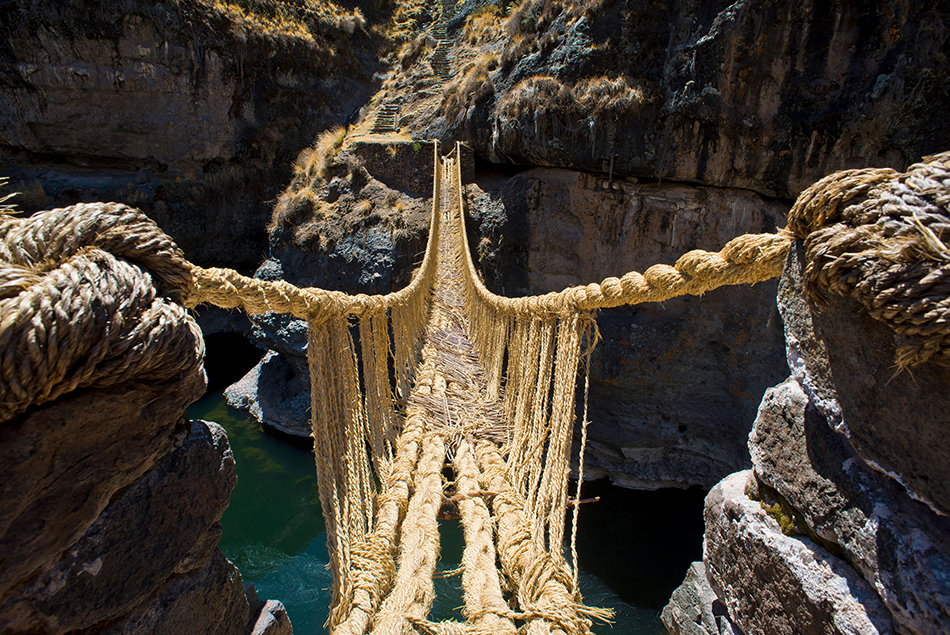
\includegraphics[width=10cm]{Immagini/Ponte_Inca}
	\caption{Ponte di corda inca sul fiume Akpurimac, Perù}	
	\label{fig:ponte_inca}
\end{figure}

Nello stesso periodo, in Tibet, Tangtong Gyalpo (1385 -- 1464) -- fisico e architetto tibetano -- costruì il primo ponte sospeso, Iron bridge (\cite{cyrus:ponte}) da cui deriva lo pseudonimo \textit{Iron Bridge Man}, sopra al fiume Kyichu, vicino a Lhasa (figura~\ref{fig:first_iron_bridge}). Questo fu il primo di una serie di ponti tibetani costruiti dal pioniere dell'ingegneria Gyalpo, principalmente localizzati nel continente cinese.

\begin{figure}
	\centering
	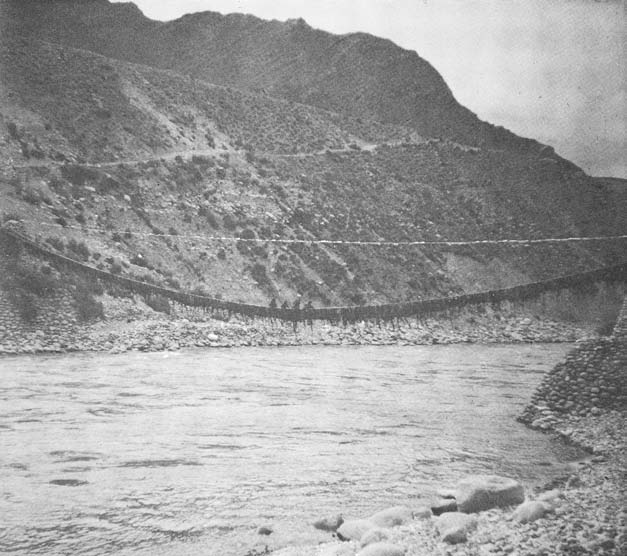
\includegraphics[width=10cm]{Immagini/Iron_Bridge_01}
	\caption{Primo ponte sospeso costruito da Gyalpo}
	\label{fig:first_iron_bridge}
\end{figure}

I ponti sospesi progettati dal fisico tibetano avevano una struttura portante formata da due lunghe catene (il cui dettaglio si può vedere in figura~\ref{fig:catena_iron_bridge}) che avevano la funzione di sorreggere, mediante altre catene, la passerella sottostante formata quasi esclusivamente da materiale ligneo (vedi figure~\ref{fig:ponte_tibetano}).

\begin{figure}
	\centering
	\subfloat[\emph{Iron bridge di Toling, Cina -- rinforzato, in seguito, da cavi in acciaio}]{
	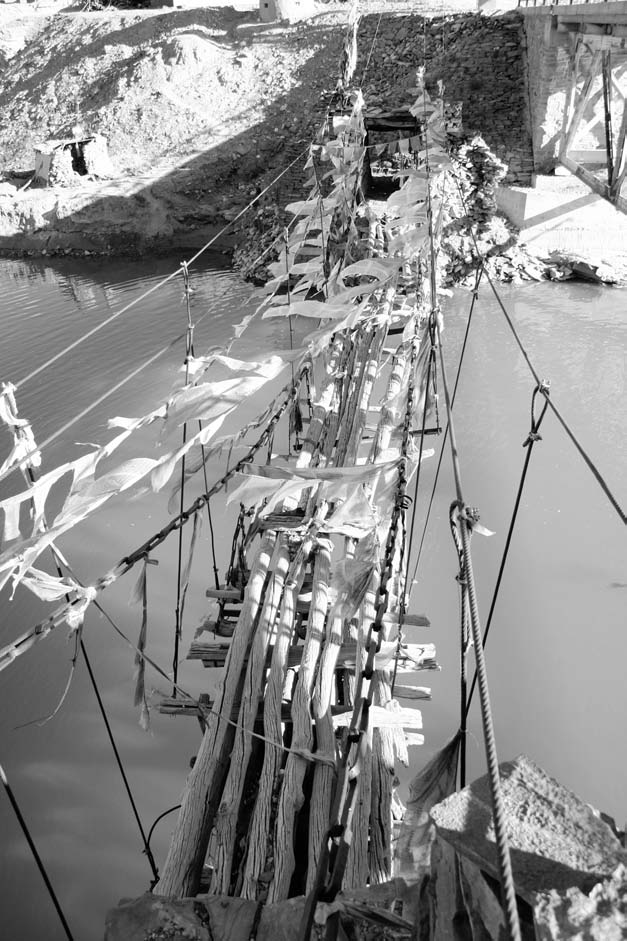
\includegraphics[width=10cm]{Immagini/Iron_Bridge}	\label{fig:iron_bridge}
}\\
	\subfloat[\emph{Catena utilizzata per la costruzione del Iron bridge}]{
	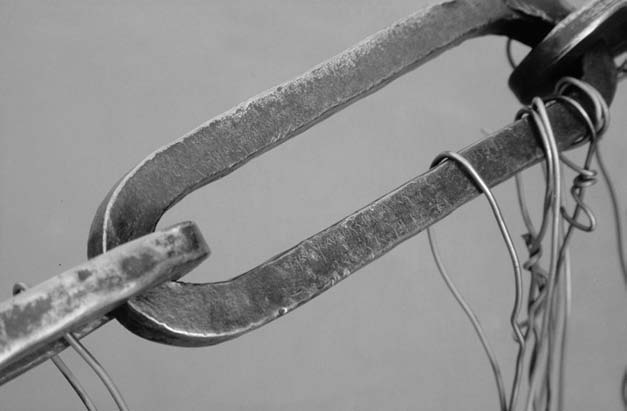
\includegraphics[width=10cm]{Immagini/Catena_Iron_Bridge}\label{fig:catena_iron_bridge}
}
	\caption{Ponte sospeso Iron bridge, Tibet}
	\label{fig:ponte_tibetano}
\end{figure}

Nonostante fossero strutture incredibili per l'epoca, questi ponti sospesi avevano una lunghezza e una portata limitata soprattutto a causa dei materiali utilizzati per la struttura portante: infatti le corde intrecciate e le catene -- benché di leghe di ferro -- non sono nemmeno paragonabili, in termini di resistenza meccanica, alle funi in uso nelle epoche successive.

Si comprende, quindi, come la consapevolezza dell'utilizzo dei cavi (intesi prima come corde e catene e in seguito come funi di acciaio)
sia da ricercarsi nell'antichità, ancora prima dello studio dello stato tensionale, risolto poi, con l'ausilio della meccanica moderna a partire da Leonardo da Vinci. 

Fu proprio da Vinci il primo a studiare la teoria delle funi, per poi essere seguito nei secoli successivi da Galileo Galilei, Huygens, Bernoulli e molti altri.
In tabella~\ref{tab:th_funi} (presa da \cite{landrini:storia}) sono riportati i contributi più significativi allo sviluppo della teoria delle funi.


\begin{table}
	\centering
	\caption{Evoluzione della teoria delle funi}
	\label{tab:th_funi}
	\begin{tabular}{p{1cm}p{3.5cm}p{5.5cm}}
		\toprule
		Anno &Autore &Oggetto\\
		\midrule
		1452 - 1519 & Leonardo da Vinci & Primi studi sulle funi\\
		1614 & Beeckman & Ponte sospeso: andamento\\&& parabolico\\
		1638 &Galileo Galilei &La parabola inestensibile\\
		1646 &Huygens &La parabola di Galileo\\&& può essere sbagliata\\
		1673 &G. Pardies &La parabola di Galileo\\&& è sbagliata\\
		1691 &Huygens, Leibniz, Bernoulli &La Catenaria inestensibile\\
		1891 &Routh &La Catenaria elastica\\
		1975 &Irvine &La Catenaria elastica sotto\\&& l'azione dei carichi concentrati	\\	
		\bottomrule
	\end{tabular}
\end{table}
%
%
%
\section{Le funi in acciaio}
Di notevole importanza per l'evoluzione della fune per uso strutturale non è solo la conoscenza matematica e fisica dettata dalla teoria dei fili, che verrà trattata nei capitoli successivi, ma è anche l'utilizzo di materiali sempre più resistenti e adatti all'uso in questione.

Ecco che si passa dall'uso di corde intrecciate e catene in ferro, all'impiego di funi in acciaio, generalmente di sezione circolare.

{\small
\begin{table}
	\centering
	\caption{Differenze tra acciaio per funi e acciaio strutturale (dolce e ad alta resistenza)\cite{gimsing:cable}}
	\label{tab:acciaio_differenze}
	\begin{tabular}{p{.21\textwidth}cccc}
		\toprule
		&Unità&Acciaio per funi&\multicolumn{2}{c}{Acciaio strutturale}\\
		&&&Dolce&Alta resistenza\\
		\midrule
		Tensione di snervamento&\si{MPa}&\num{1180}&\num{240}&\num{690}\\
		Carico di rottura a trazione&\si{MPa}&\num{1570}&\num{370}&\num{790}\\
		Deformazione a rottura&\%&\num{4}&\num{24}&-\\
		Modulo elastico&\si{GPa}&\num{205}&\num{210}&\num{210}\\
		Percentuale di carbonio presente&\%&\num{0.80}&\num{0.20}&\num{0.15}\\
		\bottomrule
	\end{tabular}
\end{table}
}

L'acciaio impiegato per le funi, a differenza di quello usato in altri ambiti, è caratterizzato da una composizione chimica con un alto contenuto di carbonio che rende la fune fino a quattro volte più resistente rispetto all'acciaio strutturale dolce\footnote{Acciaio con basso contenuto di carbonio (minore del 1\%)\cite{sito:ravaniacciai}} e fino a due volte più resistente rispetto all'acciaio ad alta resistenza rendendo, però, impossibile il collegamento dei fili mediante saldatura e creando il rischio di formazione di cricche a caldo.  

Per contro l'elevata percentuale di carbonio provoca una notevole diminuzione della duttilità del materiale riducendo a quasi un quinto la deformazione a rottura che si ha nell'acciaio strutturale dolce.

Analizzando il contenuto della tabella~\ref{tab:acciaio_differenze} della pagina successiva si evince che la resistenza a trazione dell'acciaio per funi è molto più elevata dell'acciaio per uso strutturale con un carico di rottura quasi doppio (\num{1570}\si{MPa} per la fune contro i \num{790}\si{MPa} dell'acciaio strutturale ad alta resistenza). Questa caratteristica rende la fune ideale per resistere a sforzi di trazione elevati con un impiego di materiale (e perciò di peso totale dell'opera) nettamente inferiore a strutture che impiegano altre tecnologie.
Si può notare, infine, una diminuzione del modulo elastico che passa da \num{210}\si{GPa} a \num{205}\si{GPa} il quale implica che, a parità di sforzo impresso, la deformazione aumenta (linearmente in caso di campo elastico -- lineare).

La versatilità della fune sta principalmente nel fatto di essere prefabbricata e quindi componibile a piacere: in base al diametro di cui si necessita è possibile assemblare la fune mediante l'insieme di fili.

\begin{figure}[t]
	\centering
	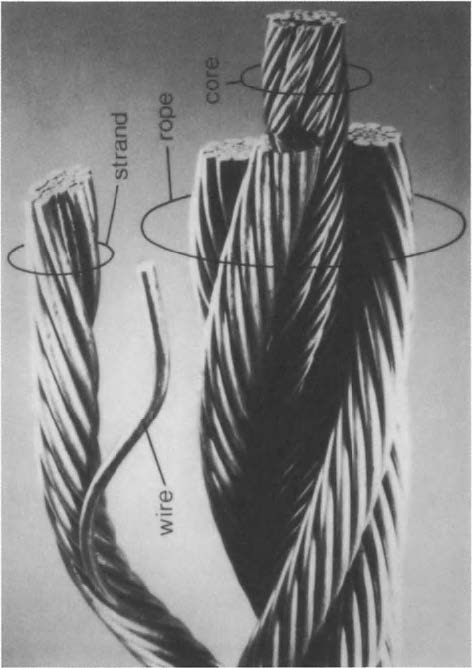
\includegraphics[width=10cm]{Immagini/Fune}
	\caption{Composizione di una fune di acciaio (\cite{costello:fune})}
	\label{fig:fune}
\end{figure}

In particolare, come descritto in figura~\ref{fig:fune}, la fune è composta come segue:
\begin{enumerate}
	\item filo (\textit{wire}): elemento base per la composizione della fune;
	\item trefolo (\textit{strand}): insieme di fili disposti in svariate forme;
	\item fune (\textit{rope}): elemento finale composto da un determinato numero di trefoli avvolti elicoidalmente attorno a un'anima centrale (\textit{core}) che può essere a sua volta un trefolo.
\end{enumerate}

\subsection{Filo}
Il filo è l'elemento alla base della fune. In base alle applicazioni il diametro del filo può variare; ad esempio, per le funi usate nei ponti moderni si possono trovare diametri di:
\begin{itemize}
	\item \num{5}\,--\,\num{5.5}\si{mm} per i cavi principali dei ponti sospesi;
	\item \num{7}\si{mm} per i cavi di ponti strallati.
\end{itemize}


\subsection{Trefolo}
Il trefolo è un insieme di fili in opportune configurazioni: i fili possono essere avvolti elicoidalmente oppure disposti in maniera parallela.
%In ambito strutturale si usa una configurazione di sette fili da \num{5}\si{mm} per un diametro nominale del trefolo di \num{15}\si{mm};

\begin{figure}[]
	\centering
	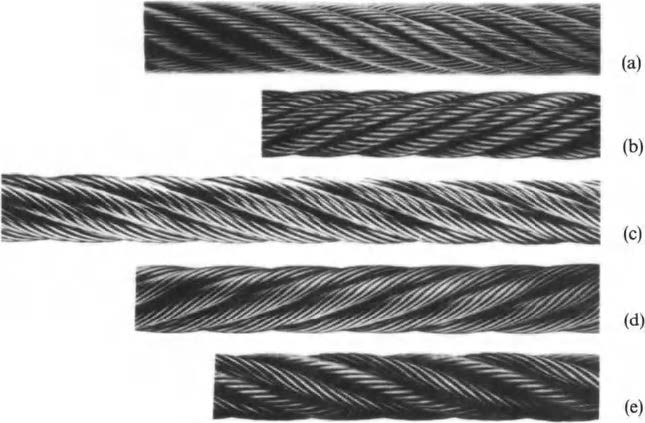
\includegraphics[width=10cm]{Immagini/Avvolgimento_Trefolo}
	\caption{Tipologie di avvolgimento dei fili che formano il trefolo [\cite{costello:fune}]}
	\label{fig:avvolgimento_trefolo}
\end{figure}

\subsubsection*{Avvolgimento elicoidale}
Per quanto riguarda l'avvolgimento elicoidale ne esistono di vari tipi: in figura~\ref{fig:avvolgimento_trefolo} sono mostrati i principali.

In particolare si differenziano tra loro per la posa (\textit{lay}) che descrive il senso di rotazione dei fili durante la costruzione del trefolo (\textit{right} o \textit{left}) e per la direzione di posa dei fili rispetto a quella del trefolo; questa può essere crociata (\textit{regular}) se i fili che compongono il trefolo sono posati nel senso opposto ai trefoli che compongono la fune oppure parallela (\textit{lang}) se i fili sono posati nello stesso verso del trefolo.

In dettaglio si ha:
\begin{description}[font=\normalfont]
	\item[(a)] \emph{Right regular lay:} i fili sono avvolti in modo tale da andare da sinistra verso destra (\textit{right}) e sono posati con senso opposto rispetto alla posa del trefolo (\textit{regular});
	\item [(b)] \emph{Left regular lay:} i fili sono avvolti da destra verso sinistra (\textit{left}) e hanno direzione opposta al trefolo (\textit{regular});
	\item [(c)] \emph{Right lang lay:} l'avvolgimento va da sinistra a destra (\textit{right}). I fili sono posati in modo concorde al senso di posa del trefolo (\textit{lang});
	\item [(d)] \emph{Left lang lay:} l'avvolgimento va da destra verso sinistra (\textit{left}). La posa avviene in maniera concorde al trefolo (\textit{lang});
	\item[(e)] \emph{Right alternate lay:} i fili hanno verso da sinistra a destra (\textit{right}) mentre la posa viene alternata tra \textit{regular} e \textit{lang}.
\end{description}
La cordatura \textit{right regular}, grazie alla posa crociata, è meno soggetta a torsioni e schiacciamenti ed è quindi la posa adatta alla maggior parte delle applicazioni.
La cordatura \textit{lang}, invece, ha una flessibilità maggiore e quindi si può flettere più facilmente, a parità di diametro, rispetto alla precedete tipologia. Tende, inoltre, a collassare in caso di eccessive rotazioni, il che la rende meno adatta per applicazioni strutturali.

In alternativa si possono sovrapporre diversi strati di fili avvolti elicoidalmente la cui anima centrale è un unico filo rettilineo.

Poiché sono presenti spazi vuoti nell'avvolgimento, quando il carico viene applicato alla fune, si ha un assestamento dei trefoli che genera una deformazione irreversibile. Per questo motivo prima dell'applicazione del carico viene effettuato un pretensionamento che ha il fine di compattare il cavo e risolvere il problema sopra descritto.

%%%%%%%%%%%%%%%%%%%%%%%%%%%%%%%%%%%%%%%%%%%%%%%%%%%%%%%%%%%%%%%%%%%%%%%%



%%%%%%%%%%%%%%%%%%%%%%%%%%%%%%%%%%%%%%%%%%%%%%%%%%%%%%%%%%%%%%%%%%%%%%%%

\subsubsection*{Locked--coil strands}
Il locked--coil strand è una tipologia di trefolo formata da due diversi tipi di fili avvolti elicoidalmente. L'anima centrale è un trefolo generico, composto da due o più strati di fili che si avvolgono ellitticamente con le pose viste sopra.
All'esterno sono posti dei particolari fili a forma di \textit{Z} che si incastrano perfettamente, diminuendo di molto gli interstizi (minori del \num{10}\%) e di conseguenza aumentando la superficie di contatto che risulta molto più continua e compatta rispetto alle altre tipologie. Questo protegge maggiormente il trefolo dalla corrosione e lo rende più resistente a pressioni laterali.

\begin{figure}
	\centering
	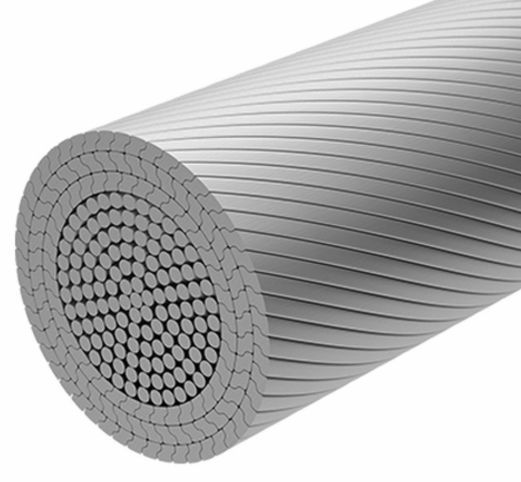
\includegraphics[width=9cm]{Immagini/Locked_coil_strands}
	\caption{Esempio di locked--coil strand}
	\label{fig:locked_coil_strands}
\end{figure}

\subsubsection*{Parallel--wire strands}
Per via della diminuzione di resistenza e rigidezza a cui sono soggette le funi ellittiche, sono stati sviluppati dei particolari trefoli composti da soli fili paralleli tra loro.

Inizialmente questa tipologia portava con se una problematica che rendeva il trefolo inutilizzabile: l'avvolgimento. Infatti, per evitare distorsioni sulla sezione durante l'avvolgimento si sarebbe dovuto avere un allungamento dei fili superiori e un accorciamento dei fili interni alla curva che, però, avrebbe generato nel materiale delle tensioni molto elevate e quindi non ammissibili.

In figura~\ref{fig:parallel_wire_strands} sono descritti i principali tipi di \emph{parallel--wire strands}; in particolare, partendo da sinistra si ha:
\begin{itemize}
	\item \emph{Regular Hexagonal}: i fili sono disposti in modo da formare un cavo di forma esagonale;
	\item \emph{Deformed Hexagonal}: rispetto a quello precedente risulta più "schiacciato" in altezza;
	\item \emph{Quasi Hexagonal}: ha una forma simile a un esagono.
\end{itemize}

In tutti i casi sopra descritti vengono impiegati fili di diametro \num{5}\si{mm}.

\begin{figure}
	\centering
	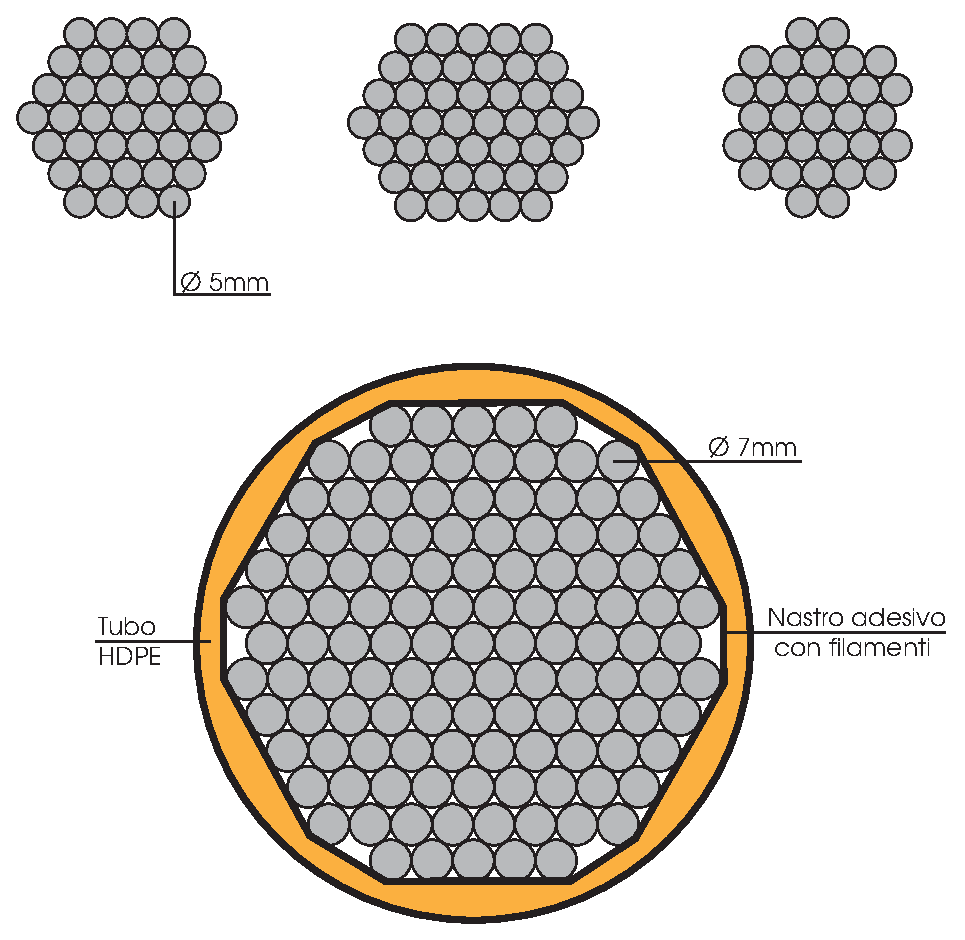
\includegraphics[width=10cm]{Immagini/Parallel_wire_strands}
	\caption{Esempi di \emph{parallel--wire strands} (in alto) e \emph{new PWS cable} (in basso)}
	\label{fig:parallel_wire_strands}
\end{figure}

Nel tempo sono state proposte varie soluzioni al problema, una delle quali è quella di inserire i fili in un involucro di polietilene (HDPE -- High Density Poly-Ethylene) che evita rotazioni e deformazioni della sezione in modo che mantenga la forma originale. Questa soluzione prende il nome di \emph{New PWS Cable} ed è stata sviluppata in Giappone negli anni '90. In figura~\ref{fig:parallel_wire_strands} (in basso) è rappresentata una sezione del cavo \textit{PWS}.



%%%%%%%%%%%%%%%%
%L'anima centrale oltre che resistere alle sollecitazioni ha il compito di mantenere in posizione i trefoli che sono all'esterno
%%%%%%%%%%%%%%%%%%


%
%
%
%I ponti sospesi sono largamente utilizzati anche in epoca moderna principalmente per il fatto che le funi sono soggette solamente a sforzi di trazione.
%Nonostante l'acciaio sia un materiale isotropo al che risponde in maniera quasi analoga per sforzi di trazione e compressione, avere uno stato tensionale di trazione elimina il problema di instabilità che caratterizza le strutture compresse. 


\section{Applicazione delle funi a strutture moderne}
L'avvento dell'acciaio consente, grazie alla sua miglior resistenza meccanica, di costruire strutture molto snelle e di lunghezze prima impensabili.
In particolare, i ponti moderni che impiegano le funi possono essere classificati in:
\begin{enumerate}
	\item ponti sospesi;
	\item ponti strallati.
\end{enumerate}

Questi si differenziano tra loro principalmente per la configurazione del sistema di funi che crea una diversificazione nelle applicazioni, in particolare nella lunghezza delle campate.

\subsection{Ponti sospesi}
I ponti sospesi sono, tra i ponti moderni, quelli che collegano distanze elevate (200 -- 2000\si{m}), motivo per cui sono largamente utilizzati sia in ambito stradale che in ambito ferroviario. 

\begin{figure}
	\centering
	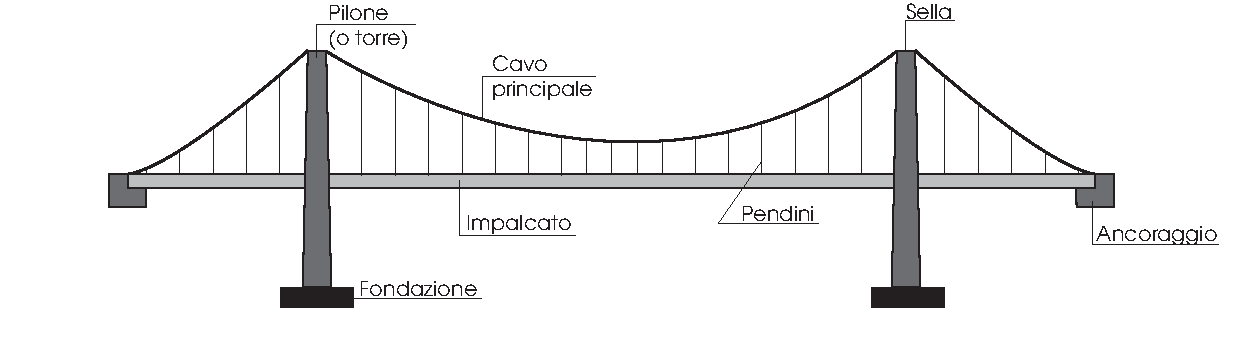
\includegraphics[width=11.8cm, keepaspectratio]{Immagini/suspension_bridge}
	\caption{Schema di un ponte sospeso}
	\label{fig:ponte_sospeso}
\end{figure}
\begin{figure}
	\centering
	
	\begin{tikzpicture}
	
	%\draw[help lines] (0,0) grid (10,5);
	\point {a}{0}{2};
	\point {b}{1}{2};
	\point {c}{2}{0};
	\point {d}{8}{0};
	\point {e}{9}{2};
	\point {f}{10}{2};
	\point {g}{8}{5};
	\point {h}{2}{5};
	
	\beam {2}{a}{h};
	\beam {2}{b}{e};
	\beam {2}{c}{h};
	\beam {2}{d}{g};
	\beam {2}{f}{g};
	
	\support {1}{b};
	\support {1}{e};
	\support {3}{c};
	\support {3}{d};
	\support {3}{a}[-45];
	\support {3}{f}[45];
	
	\internalforces{h}{g}{0}{0}[-2.5][black];

	
	
	
	
	
	
	\end{tikzpicture}
	
	
	\caption{Schema statico di un ponte sospeso}
	\label{fig:schema_statico_sospeso}
	
\end{figure}

Come descritto in figura~\ref{fig:ponte_sospeso} i ponti sospesi si compongono di:
\begin{itemize}
	\item impalcato: parte transitabile della struttura che può essere in acciaio o cemento armato e può essere pedonale, ferroviaria o stradale. L'impalcato ha anch'esso un compito di resistenza essendo dotato di rigidezza flessionale che riduce così le deformazioni del piano;
	\item sistema di cavi: elemento caratteristico dei ponti sospesi, comprende il cavo principale e i pendini (cavi verticali) e ha il compito di trasmettere gli sforzi dall'impalcato alle torri. Sotto l'effetto della forza peso tende ad acquisire una forma simile a una parabola;
	\item piloni (o torri): elementi che scaricano gli sforzi derivanti dalle funi  alle fondazioni e quindi al terreno. Sono soggetti a momento flettente, motivo per cui il cavo principale viene fatto proseguire e vincolato in appositi ancoraggi a terra. In questo modo il momento flettente generato viene equilibrato;
\end{itemize}

Difficilmente le campate risultano tutte di egual misura; infatti si predilige l'impiego di una campata centrale molto lunga e due campate laterali di lunghezza inferiore.
Nel caso di campate laterali di lunghezza uguale si otterrebbe una struttura simmetrica; ma in molti casi queste hanno lunghezze differenti dipendenti dalla morfologia del territorio.

\subsection{Ponti strallati}

\begin{figure}
	\centering
	\subfloat[\emph{Schema a ventaglio}]{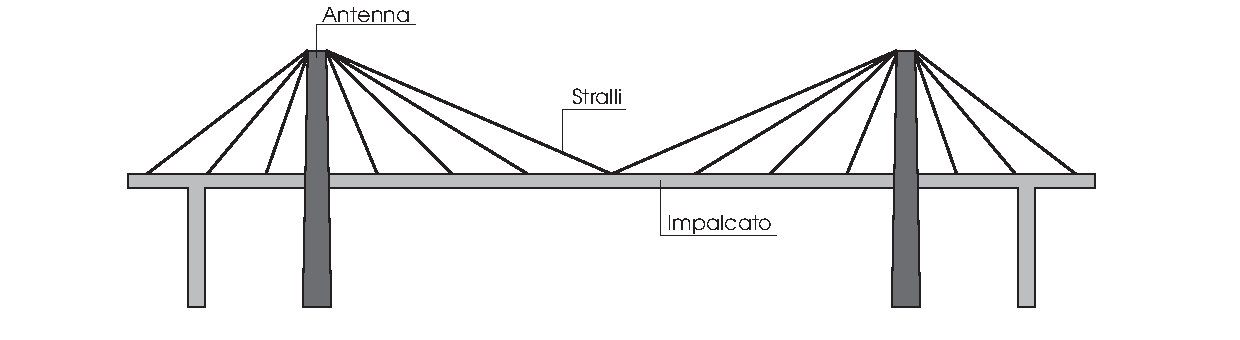
\includegraphics[width=11.8cm]{Immagini/cable_stayed_bridge_ventaglio}\label{fig:cable_stayed_ventaglio}}\\
	\subfloat[\emph{Schema a semi--ventaglio o "ventaglio modificato"}]{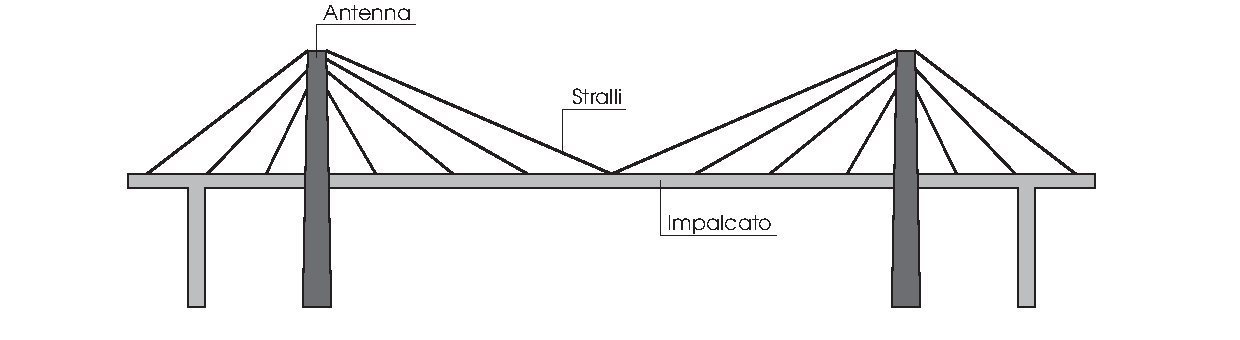
\includegraphics[width=11.8cm]{Immagini/cable_stayed_bridge_semiventaglio}\label{fig:cable_stayed_semiventaglio}}\\
	\subfloat[\emph{Schema ad arpa}]{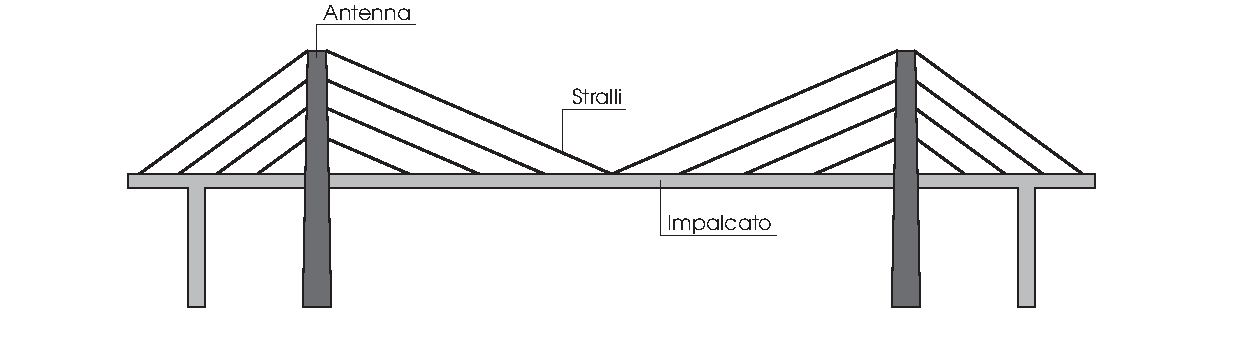
\includegraphics[width=11.8cm]{Immagini/cable_stayed_bridge_arpa}\label{fig:cable_stayed_arpa}}
	\caption{Schemi delle varie tipologie di ponti strallati}
	\label{fig:cable_stayed_bridge}
\end{figure}

\begin{figure}
	\centering
	
	\begin{tikzpicture}
	\scaling{.58};
	
	\point {a}{-5}{4};
	\point {b}{5}{4};
	\point {c}{-9}{0};
	\point {d}{9}{0};
	\point {e}{-9}{-2};
	\point {f}{9}{-2};
	
	
	\point {g2}{-8}{0};
	\point {g3}{-7}{0};
	\point {g4}{-6}{0};
	\point {g5}{-5}{-2};
	\point {g6}{-4}{0};
	\point {g7}{-3}{0};
	\point {g8}{-2}{0};
	\point {g9}{-1}{0};
	
	\point {h1}{1}{0};
	\point {h2}{2}{0};
	\point {h3}{3}{0};
	\point {h4}{4}{0};
	\point {h5}{5}{-2};
	\point {h6}{6}{0};
	\point {h7}{7}{0};
	\point {h8}{8}{0};
	
	
	\beam {2}{c}{d};
	
	\beam {2}{a}{c};
	\beam {2}{c}{e};
	\beam {2}{b}{d};
	\beam {2}{d}{f};
	\beam {2}{a}{g9};
	\beam {2}{b}{h1};
	\beam {2}{a}{g2};
	\beam {2}{a}{g3};
	\beam {2}{a}{g4};
	\beam {2}{a}{g5};
	\beam {2}{a}{g6};
	\beam {2}{a}{g7};
	\beam {2}{a}{g8};
	\beam {2}{b}{h1};
	\beam {2}{b}{h2};
	\beam {2}{b}{h3};
	\beam {2}{b}{h4};
	\beam {2}{b}{h5};
	\beam {2}{b}{h6};
	\beam {2}{b}{h7};
	\beam {2}{b}{h8};
	
	\support {1}{e};
	\support {1}{f};
	\support {3}{g5};
	\support {3}{h5};
	
	\hinge {1}{a};
	\hinge {1}{b};
	\hinge {1}{c};
	\hinge {1}{d};
	\hinge {1}{e};
	\hinge {1}{f};
	\hinge {1}{g2};
	\hinge {1}{g3};
	\hinge {1}{g4};
	%\hinge {1}{g5};
	\hinge {1}{g6};
	\hinge {1}{g7};
	\hinge {1}{g8};
	\hinge {1}{g9};
	
	\hinge {1}{h1};
	\hinge {1}{h2};
	\hinge {1}{h3};
	\hinge {1}{h4};
	%\hinge {1}{h5};
	\hinge {1}{h6};
	\hinge {1}{h7};
	\hinge {1}{h8};
	\end{tikzpicture}
		
	
	\caption{Schema statico di un ponte strallato a ventaglio}
	\label{fig:schema_statico_ventaglio}
\end{figure}

In epoca moderna i ponti strallati sono i più usati per congiungere punti posti a distanze medio -- lunghe (intorno ai 1000\si{m}).
Si differenziano, dai ponti sospesi, in maniera molto chiara per il sistema di cavi, detti \emph{stralli}, che - una volta posati - risultano quasi rettilinei.

In questa configurazione l'impalcato è sorretto dagli stralli, che risultano soggetti a uno sforzo di trazione e inducono uno stato di compressione nella torre e nell'impalcato.

La compressione che si genera nell'impalcato provoca l'impossibilità di raggiungere luci elevate con questa tipologia di ponte. Per colmare, in parte, il problema è consigliato ancorare gli stralli di riva a terra in modo da limitare il carico sull'impalcato.



In figura~\ref{fig:cable_stayed_bridge} sono rappresentate le diverse configurazioni degli stralli; infatti, in base al collegamento dei cavi con la torre si possono ottenere diverse tipologie di ponti strallati.
\subsubsection{Schema a ventaglio}

Nel caso in cui i cavi convergano in un solo punto alla sommità della torre si parla di \emph{schema a ventaglio} (figura~\ref{fig:cable_stayed_ventaglio}).

Questa disposizione risulta molto efficiente grazie al fatto che avvicinandosi alla torre l'angolo compreso tra l'impalcato e lo strallo aumenta; ne consegue che la componente orizzontale degli sforzi assorbita dall'impalcato diminuisce. 

Per motivi tecnici, in presenza di molti stralli, risulta difficoltoso ancorare i cavi disposti a ventaglio alla torre. Per questo si utilizza lo schema a \emph{semi--ventaglio}.

\subsubsection{Schema a semi--ventaglio}
Usato nel caso di un numero elevato di cavi, è simile allo schema a ventaglio, mantenendone le particolarità positive e risolvendo il problema dell'ancoraggio andando a distribuire l'attacco degli stralli nella parte superiore della torre (come si può vedere in figura~\ref{fig:cable_stayed_semiventaglio}).

\subsubsection{Schema ad arpa}
La disposizione ad arpa (figura~\ref{fig:cable_stayed_arpa}) è composta da stralli tutti paralleli tra loro, implicando così, la distribuzione degli ancoraggi lungo tutta la torre.
Le distanze tra gli ancoraggi verticali e orizzontali sono tra loro proporzionali.
Questo schema è quello meno efficiente tra quelli visti poiché il sistema di cavi paralleli genera uno stato tensionale di compressione notevole nell'impalcato che lo rende non adatto a coprire luci elevate.







 



%
%
%
\cleardoublepage
%
%
%
\cleardoublepage
\chapter{Teoria dei fili ideali}\label{chapter:teoria_fili}
Nella trattazione analitica (derivante da \cite{siboni:funi}), quando si parla di filo (o fune), si intende un solido la cui lunghezza longitudinale sia molto maggiore della lunghezza caratteristica della sezione (diametro o diagonale, in base alla forma), con scarsa resistenza a flessione e torsione e che sopporti solo sforzi di trazione.

In questo modo è possibile descrivere il filo mediante una curva di parametrizzazione

\begin{equation*}
	P=P(\lambda) \quad \lambda\in[\lambda_1, \lambda_2]
\end{equation*}
La curva deve risultare sufficientemente regolare e di classe almeno $C^2$.
Per definizione, i punti $P(\lambda_1)$ e $P(\lambda_2)$ vengono detti \emph{estremi del filo}.

La teoria qui riportata fa riferimento ai cosiddetti \emph{fili ideali}, definiti da due caratteristiche principali:
\begin{enumerate}
	\item configurazioni ammissibili;
	\item reazioni vincolari.
\end{enumerate}

\section*{Configurazioni ammissibili}
Un filo ideale può assumere qualsiasi configurazione descritta da una curva $C^2$ regolare (o biregolare) di lunghezza $L$ assegnata. Questo significa:
\begin{itemize}
	\item la curvatura $1/\,\rho$ e la torsione $1/\,\sigma$ possono assumere valori arbitrari come si deduce dalle formule di Frenet -- Serret
	\begin{equation*}
		\dfrac{d\hat{\tau}}{ds} = \dfrac{1}{\rho}\,\hat{n} \hspace*{2cm} \dfrac{d\hat{b}}{ds} = - \dfrac{1}{\sigma}\,\hat{n}
	\end{equation*}
	dove $s$ è l'ascissa curvilinea e $\hat{\tau}$, $\hat{n}$, $\hat{b} = \hat{\tau} \wedge \hat{n}$ sono rispettivamente i versori tangente, normale e binormale alla curva nella posizione $P(s)$.

	L'arbitrarietà di questi valori rende il filo ideale perfettamente deformabile sia a flessione che a torsione, cosa che non accade in una fune reale: infatti, curvature molto grandi, genererebbero un momento flettente elevato nelle fibre interne del materiale che causerebbe la rottura dell'elemento. In particolare, curvatura e momento flettente sono legati dalla seguente legge caratteristica
	\[
	M = E\,I\,\chi
	\]
	dove $E$ è il modulo elastico del materiale, $I$ è il momento di inerzia della sezione e $\chi$ è la curvatura.

	Si assume, quindi, rigidezza flessionale nulla ($E\,I\simeq 0$).
	\item la lunghezza $L$ del filo è costante; le configurazioni $P(\lambda)$ devono soddisfare la condizione di \emph{inestensibilità}
	\[
	\int_{\lambda_1}^{\lambda_2} \left| \dfrac{dP}{d\lambda}(\lambda) \right|\,d\lambda = \int_{\lambda_1}^{\lambda_2} [\dot{P}(\lambda)^2]^{1/2}\, d\lambda = L = cost.
	\]
	la cui impone che il filo, anche se sottoposto a sollecitazioni, non subisce variazioni di lunghezza. Anche in questo caso si tratta di una approssimazione della realtà poiché una fune reale, soggetta a sollecitazioni più o meno grandi, si allunga secondo il legame costitutivo del materiale.

	La condizione di inestensibilità postula una rigidezza assiale infinita ($E\,A \to \infty$).
\end{itemize}

\section*{Reazioni vincolari}
Il filo ideale sottoposto alle sollecitazioni reagisce internamente con delle reazioni vincolari interne.

Considerando un intervallo $\lambda\in[\lambda_1, \lambda_2]$ si postula che le reazioni vincolari interne ad un tratto di filo (ad esempio $P(\lambda) - P(\lambda_2)$) si riducano a una unica reazione vincolare applicata in $P(\lambda)$. Questa forza, indicata con $\overline{T}(\lambda)$, prende il nome di \emph{tensione del filo} e risulta essere tangente alla curva in $\lambda$ (vedi figura~\ref{fig:tensione_filo}).

\begin{figure}[ht]
		\centering
		
		\subfloat[\emph{Tensione in un tratto di filo}\label{fig:tensione_filo}]{
		\begin{tikzpicture}[scale=.8]
		
			
			
			\draw[line width=1pt] (0,0)node [left] {$P(\lambda_1)$} .. controls ++(1.5,3) and ++(.1,-2) .. (10,4) node [right] {$P(\lambda_2)$}
			node[sloped, pos=.3, anchor=south west,
			minimum height=(10.5)*0.3cm,minimum width=(10.5)*.3cm](p){};
			
			\path (p.south west)%
		%	edge[-stealth',blue] node[left] {$\vec{ n}$} (p.north west)
			edge[-stealth',blue, thick] node[pos=1, above] {$\overline{T}(\lambda)$} (p.south east);
			
			\node at (p.south west) [below] {$P(\lambda)$};
			
			
			
		
		
		
		
 						\end{tikzpicture}}
 		
 		\subfloat[\emph{Estensione del postulato a una fune ideale}\label{fig:tensione_fune_ideale}]{
 		
 		
 		
 		
 \begin{tikzpicture}[scale=.9]
  
 \draw plot  [smooth, tension=1] coordinates {(0,0) (1,.3) (3,.6)};
 \begin{scope}[shift={(0,-1)}]
 \draw plot  [smooth, tension=1] coordinates {(0,0) (1,.3) (3,.6)};
 \end{scope}
 
 \draw (0,0) to [out=-20, in=40] (0,-1);
 \draw (0,0) to [out=-145, in=130] (0,-1);
 
 \draw (3,.6) to [out=-20, in=40] (3,-.4);
 \draw [dashed] (3,.6) to [out=-145, in=130] (3,-.4);
 
 \draw [-stealth', blue] (3,.1) --([turn] 8:1) node [above] {\small$\overline{T}(\lambda)$};
 \draw [-stealth, red] (0,-.5) --([turn] 290:1) node [below] {\small$\overline{T}(\lambda_1)$};
 
 \node at (0,0) [left] {$P(\lambda_1)$};
 \node at (3,.6) [above] {$P(\lambda)$};
 
 \begin{scope}[shift={(9,0.35)}, yscale=1, xscale=-1]
 \draw plot  [smooth, tension=1] coordinates {(0,0) (1,.3) (3,.6)};
 \begin{scope}[shift={(0,-1)}]
 \draw plot  [smooth, tension=1] coordinates {(0,0) (1,.3) (3,.6)};
 \draw [-stealth, red] (0,.5) --([turn] 100:1) node [below] {\small$\overline{T}(\lambda_2)$};
 \end{scope}
 
 \draw [dashed](0,0) to [out=-20, in=40] (0,-1);
 \draw [] (0,0) to [out=-145, in=130] (0,-1);
 
 \draw (3,.6) to [out=-20, in=40] (3,-.4);
 \draw [] (3,.6) to [out=-145, in=130] (3,-.4);
 
 \draw [-stealth', blue] (3,.1) --([turn] -8:1) node [above] {\small$-\overline{T}(\lambda)$};

 
 \node at (0,0) [right] {$P(\lambda_2)$};
 \node at (3,.6) [above] {$P(\lambda)$};
 \end{scope}
 \end{tikzpicture}


}
		
		
		
		
		
		
		
		
		
		\caption{Tensione in un tratto di filo}
		\label{fig:tensione_fune}
		
	\end{figure}
	
	
	


Estendendo quanto appena visto a una fune ideale di sezione non puntuale e tagliando in corrispondenza di $P(\lambda)$, per il \emph{principio di azione e reazione}, il tratto residuo genera una tensione uguale ed opposta, come mostrato in figura~\ref{fig:tensione_fune_ideale}.

Poiché il filo ideale è un elemento a sezione puntuale, il momento delle reazioni vincolari interne agenti su ogni sezione -- rispetto al baricentro -- risulta nullo. Ne consegue la condizione di \emph{perfetta flessibilità}, descritta poc'anzi, che è rafforzata dalla richiesta di  resistenza nulla a sforzi di taglio da parte del filo dovuta al fatto che la tensione è tangente al supporto del filo.

Nella realtà, avendo il filo un diametro non infinitesimo, il momento generato dalle reazioni vincolari interne è, generalmente, diverso da zero.

Infine, l'arbitrarietà del valore della tensione (che si impone di sola trazione) comporterebbe un carico di rottura del filo infinito, condizione che non è assolutamente applicabile in caso di fune reale.

\subsection*{Osservazione}
Mentre la tensione $\overline{T}(\lambda)$ è definita come una reazione vincolare interna, agli estremi, i termini $\overline{T}(\lambda_1)$ e $\overline{T}(\lambda_2)$ sono descritti come forze attive che interagiscono con l'esterno come, per esempio, un vincolo; in questo caso le tensioni $\overline{T}(\lambda_1)$ e $\overline{T}(\lambda_2)$ si identificano con i \emph{cimenti dinamici} (o, in particolare, statici).

Definito il triedro di Frenet in un punto $P(\lambda)$ della curva, si può riscrivere la tensione come
\[
	\overline{T}(\lambda) = T(\lambda)\,\hat{\tau}(\lambda)
\]
dove
\[
T(\lambda) = \left|\overline{T}(\lambda)\right|\geq 0 \quad \lambda\in[\lambda_1, \lambda_2]
\]

\section{Sollecitazioni esterne}
Esistono due diverse tipologie di sollecitazioni che possono essere applicate al filo:
\begin{itemize}
	\item concentrate: sono applicate in un punto singolo del filo e sono descritte da un vettore;
	\item distribuite: sono applicate lungo un tratto (oppure tutto) di filo e sono descritte da una densità di forza per unità di lunghezza $\overline{f}(s)$. Preso un tratto infinitesimo di filo di lunghezza $ds$, la forza che agisce sul tratto considerato vale
	\[
		d\overline{F}(s) = \overline{f}(s)\,ds \quad s\in[0,L]
	\]
	ove $s$ è la \emph{ascissa curvilinea} che descrive il filo di intervallo $[0,L]$.
	In generale, le sollecitazioni sono funzione di posizione e velocità oltre che del tempo
	\[
	\overline{F} = \overline{F}(t, P, \dot{P})
	\]
\end{itemize}

\section{Condizione di equilibrio}
Per un sistema costituito da $N$ punti materiali ${P_1, \dots, P_N}$ soggetto a sollecitazioni $\overline{F}_i (t, P_i, \dot{P}_i),~ i=1,\dots,N$ la configurazione $P_0$ è di equilibrio \emph{se e solo se} la quiete in $P_0$, definita come
\[
P(t) = P_0\quad \forall t\in\mathbb{R},
\]
è un \emph{moto naturale} del sistema, cioè è soluzione delle equazioni del moto.

Il postulato delle reazioni vincolari in termini generali è descritto dalla seguente equazione
\[
m_i\,\ddot{P}_i = \overline{F}_i(t,P_i(t), \dot{P}_i(t)) + \overline{\Phi}_i\qquad i=1,\dots,N
\]
Applicandolo alla configurazione $P_0$, indicata precedentemente come in quiete, si ha
\begin{equation}
	\label{eq:equilibrio_p0}
	0 = \overline{F}_i (t, P_0, 0) + \overline{\Phi}_i\qquad i = 1,\dots, N\quad\forall t\in\mathbb{R}
\end{equation}
dove le reazioni vincolari $\overline{\Phi}_i$ devono essere quelle effettivamente esplicabili dai vincoli.

L'equazione \eqref{eq:equilibrio_p0} equivale alla \emph{prima equazione cardinale della statica}; definito un polo $O\in\mathbb{E}^3$, la \emph{seconda equazione cardinale della statica}, che deriva esplicitamente dalla prima, risulta
\begin{equation*}
	0 = (P_i - O)\wedge\overline{F}_i(t,P_0, 0) + (P_i - O)\wedge\overline{\Phi}_i\qquad i=1,\dots,N\quad\forall t\in\mathbb{R}
\end{equation*}
Allora si può dire che, \emph{condizione necessaria e sufficiente} perché $P_0$ sia un equilibrio del sistema è che siano valide le equazioni cardinali della statica, in conformità con le reazioni vincolari esplicate dai vincoli.

Per quanto riguarda un corpo continuo come un filo, si dice che:
\begin{quotation}
	una configurazione del filo è in equilibrio se e solo se sono soddisfate, per mezzo di reazioni vincolari esplicabili dai vincoli, le equazioni cardinali della statica \textbf{per ogni tratto di fune}.\footnote{citato da \cite{siboni:funi}}
\end{quotation}

\section{Equazioni cardinali della statica per un elemento di filo}




\begin{figure}
	\centering
	
	\begin{tikzpicture}[scale=.6]
	
	\draw [thick] (0,0) .. controls (5,-.5) .. (10,.5);
	
	
	
	\draw [-latex, thick] (0,-.25) -- ++([turn] 75:-1.5) node [above left] {$-\overline{T}(s)$};
	
	\draw [-latex, thick] (10,.25) -- ([turn] 12:2) node [above right] {$\overline{T}(s + \delta s)$};
	
	
	
	
	\draw [thick](0,-.5) node [below] {$P(s)$} .. controls (5,-1)..(10,0) node [below right] {$P(s+\delta s)$};
	
	\draw[thick] (0,0) .. controls (.2,-.18) and (.2,-.36) .. (0,-.5);
	\draw[thick] (0,0) .. controls (-.2,-.18) and (-.2,-.36) .. (0,-.5);
	
	\draw [thick](10,0.5) .. controls (10.1,.3) and (10.1,.1) .. (10,0);
	\draw [thick, dashed](10,0.5) .. controls (9.9,.3) and (9.9,.1) .. (10,0);
	
	
	
	\begin{scope}[shift={(0,1.3)}]
	\draw [thick]  (.15,0) .. controls (5,-.5) .. (9.7,.49);
	\draw [forcedist=.75cm]  (0,0) .. controls (5,-.5) ..(10,.5);
	\node  at (5,0.2) {$\overline{f}(\xi)$};
	\end{scope}
	
	
	\end{tikzpicture}
	
	\caption{Forze esterne agenti su un tratto di filo}
	\label{fig:forze_filo}
	
\end{figure}




\subsection{Prima equazione cardinale della statica}

Si consideri un tratto di filo compreso fra $P(s)$ e $P(s + \delta s)$ (figura~\ref{fig:forze_filo}); per l'equilibrio è necessario che il vettore risultante di tutte le sollecitazioni agenti sul tratto di filo sia nullo
\[
\overline{T}(s+\delta s) - \overline{T}(s) + \int_s^{s+\delta s} \overline{f}(\xi)\,d\xi = 0
\]
Proiettando la densità di forza lungo un generico versore $\hat{e}_i$ e applicando il teorema del valor medio, essendo $\overline{f}(\xi)$ una funzione continua nell'intervallo $\xi\in [s, s +\delta s]$, si può scrivere
\[
\hat{e}_i \cdot \int_s^{s+\delta s} \overline{f}(\xi)\,d\xi = \int_s^{s+\delta s} \hat{e}_i\cdot \overline{f}(\xi)\,d\xi = \delta s\,\hat{e}_i\cdot\overline{f}(s+ \theta_i\,\delta s)
\]
con $\theta_i\in (0,1)$ opportuno. Generalizzando per le tre direzioni $1, 2, 3$ e sostituendo nell'equazione si ottiene
\begin{equation*}
\overline{T}(s+\delta s) - \overline{T}(s) + \delta s\,\sum_{i=1}^3 \hat{e}_i\cdot \overline{f}(s+\theta_i\,\delta s)\,\hat{e}_i = 0
\end{equation*}

A questo punto, dividendo entrambi i membri per $\delta s$ e calcolando il seguente limite
\[
\lim_{\delta s\to 0} \left[ \dfrac{\overline{T}(s+\delta s)-\overline{T}(s)}{\delta s} + \sum_{i=1}^3 \hat{e}_i\cdot \overline{f}(s+\theta_i\,\delta s)\,\hat{e}_i \right] = 0
\]
si ha che siccome $\overline{f}$ è una funzione continua, detto limite esiste e vale
\[
\lim_{\delta s \to 0} \overline{f}(s+\theta_i\,\delta s) = \lim_{\delta s \to 0} \overline{f}(s+\delta s) = \overline{f}(s)
\]
da cui
\[
\lim_{\delta s \to 0} \sum_{i=1}^3 \hat{e}_i\cdot \overline{f}(s+\theta_i\,\delta s)\,\hat{e}_i = \sum_{i=1}^3 \hat{e}_i\cdot \overline{f}(s)\,\hat{e}_i = \overline{f}(s)
\]
La definizione di limite, inoltre, assicura che
\[
\lim_{\delta s \to 0} \dfrac{\overline{T}(s+\delta s)-\overline{T}(s)}{\delta s} = \dfrac{d\overline{T}}{ds}(s)
\]
In definitiva, la \textbf{prima equzione cardinale della statica} si riscrive nella seguente forma
\begin{equation}
\label{eq:prima_eq_cardinale_statica}
\dfrac{d\overline{T}}{ds}(s) + \overline{f}(s) = 0\qquad \forall s \in (s_1, s_2)
\end{equation}
che risulta una equazione differenziale nella coordinata $s$.

\subsection{Seconda equazione cardinale della statica}
Scegliendo come polo per il calcolo del momento angolare il punto $P(s)$, la seconda equazione della statica si può scrivere come
\[
[P(s+\delta s) - P(s)] \wedge \overline{T}(s+\delta s) + \int_s^{s+\delta s} [P(\xi) - P(s)]\wedge \overline{f}(\xi)\,d\xi = 0
\]
Come fatto in precedenza, si proietta l'equazione lungo i versori degli assi coordinati e si applica il teorema del valor medio
\begin{align*}
&\hat{e}_i \cdot \int_s^{s+\delta s} [P(\xi) - P(s)]\wedge \overline{f}(\xi)\,d\xi =\\ =&\int_s^{s+\delta s} \hat{e}_i \cdot [P(\xi) - P(s)]\wedge \overline{f}(\xi)\,d\xi =\\=& \delta s\,\hat{e}_i \cdot [P(s+\zeta_i\,\delta s) - P(s)] \wedge \overline{f}(s+\zeta_i\,\delta s)
\end{align*}
ove $\zeta_i \in (0,1)$ è un opportuno scalare. Sostituendo e sommando vettorialmente lungo le tre direzioni si ottiene
\begin{align*}
&[P(s+\delta s) - P(s)] \wedge \overline{T}(s+\delta s) +\\+& \delta s\,\sum_{i=1}^3 \hat{e}_i \cdot [P(s + \zeta_i\,\delta s) - P(s)]\wedge \overline{f}(s + \zeta_i\,\delta s)\,\hat{e}_i = 0
\end{align*}
Si divide, quindi, per la lunghezza $\delta s$ e si calcola il limite per $\delta s$ tendente a zero
\begin{align*}
&\lim_{\delta s\to 0} \left[ \dfrac{P(s+\delta s) - P(s)}{\delta s} \wedge \overline{T}(s + \delta s)\right] +\\
+&\lim_{\delta s\to 0} \,\sum_{i=1}^3 \hat{e}_i \cdot [P(s+\zeta_i\,\delta s) - P(s)]\wedge \overline{f}(s+\zeta_i\,\delta s)\,\hat{e}_i = 0
\end{align*}
Il secondo termine si annulla, poiché
\begin{align*}
&\lim_{\delta s\to 0} \hat{e}_i \cdot [P(s + \zeta_i\,\delta s) - P(s)] \wedge \overline{f}(s+\zeta_i\,\delta s) =\\
=& \lim_{\delta s \to 0} \hat{e}_i \cdot [P(s + \delta s) - P(s)] \wedge \overline{f}(s+\delta s) =\\
=& \hat{e}_i \cdot [P(s) - P(s)]\wedge \overline{f}(s) = 0
\end{align*}
mentre il primo termine
\begin{align*}
&\lim_{\delta s \to 0} \dfrac{P(s+\delta s) - P(s)}{\delta s} = \dfrac{dP}{ds}(s)\\[1.5ex]
&\lim_{\delta s \to 0} \overline{T}(s+\delta s) = \overline{T}(s)
\end{align*}
Allora, \textbf{seconda equazione cardinale della statica} riscritta in forma locale è
\begin{equation}
\label{eq:seconda_eq_cardinale_statica}
\dfrac{dP}{ds}(s) \wedge \overline{T}(s) = 0\qquad \forall s\in (s_1, s_2)
\end{equation}

\subsubsection*{Osservazione}
Ricordando la definizione del versore tangente
\[
\hat{\tau}(s) = \dfrac{dP}{ds}(s)
\]
la \eqref{eq:seconda_eq_cardinale_statica} assicura, grazie all'annullarsi del prodotto vettoriale, che la tensione $\overline{T}(s)$ sia tangente al filo
\[
\overline{T}(s) = T(s)\,\dfrac{dP}{ds}(s) = T(s)\,\hat{\tau}(s)
\]

Le sole equazioni cardinali della statica \eqref{eq:prima_eq_cardinale_statica} e \eqref{eq:seconda_eq_cardinale_statica} descrivono una \emph{condizione necessaria ma non sufficiente} per l'equilibrio del filo.

La sufficienza della suddetta condizione viene garantita richiedendo che le tensioni si mantengano di segno non negativo; perciò
\[
T(s)\geq 0\qquad \forall s\in(s_1, s_2),
\]
dove le tensioni sono dirette in modo concorde all'ascissa curvilinea $s$.

In definitiva, nel caso di filo soggetto a sollecitazioni distribuite di densità $\overline{f}(s)$ continua nell'intervallo $(s_1, s_2)$, \emph{condizione necessaria e sufficiente per l'equilibrio del filo} è che si soddisfino le seguenti relazioni
\begin{equation}
	\label{eq:cns_equilibrio}
	\begin{cases}
		\dfrac{d\overline{T}}{ds}(s) + \overline{f}(s) = 0\\
		\overline{T}(s) = T(s)\,\dfrac{dP}{ds}(s)\\
		T(s) \geq 0
	\end{cases}
	\quad \forall s \in(s_1, s_2)
\end{equation}

\section{Equazioni intrinseche dell'equilibrio}
Nelle ipotesi di curva biregolare  e di modulo della tensione  $T(s)$ strettamente positivo,  si può ridurre il sistema \eqref{eq:cns_equilibrio} a un'unica equazione
\begin{equation}
	\label{eq:equzione_indefinita_equilibrio}
	\dfrac{d}{ds}(T\,\hat{\tau}) + \overline{f}(s) = 0
\end{equation}
detta \emph{equazione indefinita di equilibrio}. Sviluppando la derivata del prodotto presente nel primo termine si ottiene infatti
\[
	\dfrac{dT}{ds}\,\hat{\tau} + T\,\dfrac{d\hat{\tau}}{ds} + \overline{f}(s) = 0
\]
e ricordando la definizione di curvatura che lega la derivata del versore tangente al versore normale
\[
	\dfrac{dT}{ds}\,\hat{\tau} + T\,\dfrac{1}{\rho}\,\hat{n} + \overline{f}(s) = 0
\]
Proiettando l'equazione appena ricavata lungo i versori che formano il triedro di Frenet si ottengono le \emph{equazioni intrinseche dell'equilibrio} per il tratto di filo considerato
\begin{equation}
	\begin{cases}
		\dfrac{dT}{ds} + \hat{\tau}\cdot \overline{f}(s)=0\\[2ex]
		\dfrac{T}{\rho} + \hat{n}\cdot \overline{f}(s)=0\\[2ex]
		\hat{b}\cdot \overline{f}(s)=0
	\end{cases}
\end{equation}

\subsection*{Osservazione}
La densità di forza distribuita $\overline{f}(s)$, finora scritta come funzione della sola variabile s, è in realtà una funzione nota dipendente non solo dall'ascissa curvilinea $s$ ma anche dalla parametrizzazione $P(s)$ e del versore tangente $\hat{\tau}(s)$; Si considera quindi
\[
\overline{f} = \overline{f}	(s, P(s), \hat{\tau}(s))
\]

Nella trattazione seguente si considererà implicita la dipendenza da $s$ delle funzioni tensione, versore tangente e densità di sollecitazione.

\section{Equazioni di equilibrio ridotte a forma normale}
Sia $T(s)>0\quad\forall s \in[s_1, s_2]$ e derivabile nello stesso intervallo; l'equazione indefinita di equilibrio \eqref{eq:equzione_indefinita_equilibrio} può essere riscritta come
\begin{equation}
	\label{eq:equazione_indefinita_equilibrio_1}
	\dfrac{dT}{ds}\,\hat{\tau} + T\,\dfrac{d\hat{\tau}}{ds}+ \overline{f} = 0
\end{equation}

Moltiplicando scalarmente i termini per il versore tangente si ha
\[
	\dfrac{dT}{ds}\,\hat{\tau}^2  + \overline{f}\cdot\hat{\tau} = 0
\]
e, per ottenere la variazione di $T$ in $s$ è sufficiente dividere per $\hat{\tau}^2$ e portare il secondo termine a secondo membro
\[
\dfrac{dT}{ds} = -\dfrac{\overline{f}\cdot\hat{\tau}}{\hat{\tau}^2}	
\]
Sostituendo quanto appena ricavato nella \eqref{eq:equazione_indefinita_equilibrio_1} si ottiene
\[
	-\dfrac{\overline{f}\cdot\hat{\tau}}{\hat{\tau}^2}\,\hat{\tau} + T\,\dfrac{d\hat{\tau}}{ds}+ \overline{f} = 0
\]
e riorganizzando il tutto
\[
\dfrac{d\hat{\tau}}{ds} = \dfrac{1}{T} \left(-\overline{f} + \dfrac{\overline{f}\cdot\hat{\tau}}{\hat{\tau}^2}\,\hat{\tau}\right)
\]

Ricordando, inoltre, la definizione di $\hat{\tau}$ si ottiene un sistema di 7 equazioni in 7 incognite ($P, T, \hat{\tau}$) funzioni di $s$
\begin{equation}
\label{eq:sistema_risolvente_generale}
	\begin{aligned}[c]
		\begin{cases}
			\dfrac{dP}{ds} = \hat{\tau}\\[2ex]
			\dfrac{d\hat{\tau}}{ds} = \dfrac{1}{T} \left(-\overline{f} + \dfrac{\overline{f}\cdot\hat{\tau}}{\hat{\tau}^2}\,\hat{\tau}\right)\\[2ex]
			\dfrac{dT}{ds} = -\dfrac{\overline{f}\cdot\hat{\tau}}{\hat{\tau}^2}
		\end{cases}
	\end{aligned}
	\qquad 
	\begin{aligned}
		&\forall s\in[s_1, s_2]\\
		& P\in\mathbb{R}^3\\
		&\hat{\tau} \neq 0
	\end{aligned}
\end{equation}

Moltiplicando scalarmente la seconda delle \eqref{eq:sistema_risolvente_generale} per $\vtau$ 
\[
 \vtau\cdot\dfrac{d\vtau}{ds} = \dfrac{1}{T}\left( -\overline{f}\cdot\vtau + \overline{f}\cdot\vtau\,\dfrac{\vtau^2}{\vtau^2}\right) = 0
\]
risulta un prodotto scalare identicamente nullo. Si può scrivere allora
\[
 \vtau\cdot\dfrac{d\vtau}{ds} = \dfrac{1}{2}\,\dfrac{d}{ds}(\vtau^2) = 0\quad \Longrightarrow\quad \vtau^2 = cost.
\]

La definizione di \emph{versore} impone che
\[
\left| \hat{\tau}(s)\right| = 1 \qquad \forall s\in[s_1, s_2]
\]
il che assicura, in ogni punto intermedio $s_1<s_0<s_2$
\[
	\left| \hat{\tau}(s_0)\right| = 1 
\]
e perciò, fissando il versore in $s_0$
\[
\hat{\tau}(s_0)= \hat{\tau}_0,\qquad \left|\hat{\tau}_0\right|^2 = 1
\]
essendo $\vtau^2$ costante, si garantisce la validità del teorema di esistenza e unicità della soluzione.

Applicando, così, le \textbf{condizioni iniziali} si perviene al seguente problema di Cauchy
\begin{equation}
	\label{eq:problema_cauchy}
	\begin{cases}
		\dfrac{dP}{ds} = \hat{\tau}\\[1.5ex]
		\dfrac{d\hat{\tau}}{ds} = \dfrac{1}{T} \left(-\overline{f} + \dfrac{\overline{f}\cdot\hat{\tau}}{\hat{\tau}^2}\,\hat{\tau}\right)\\[1.5ex]
		\dfrac{dT}{ds} = -\dfrac{\overline{f}\cdot\hat{\tau}}{\hat{\tau}^2}\\[1.5ex]
		P(s_0) = P_0\\
		\hat{\tau}(s_0)= \hat{\tau}_0\\
		T(s_0)=T_0
	\end{cases}
\end{equation}
ove la funzione nota $\overline{f}\in C^1$ in $s$, $P$, $\hat{\tau}$ e il dominio di definizione è
\[
\Omega = \left\{(s, P, \vtau, T)\in \mathbb{R}\times\mathbb{R}^3\times \mathbb{R}^3\texttt{\textbackslash}\left\{0\right\}\times \mathbb{R}^+\right\}
\]

Il teorema di esistenza e unicità applicato al problema di Cauchy \eqref{eq:problema_cauchy} assicura che la soluzione massimale esiste ed è unica.
La soluzione ricercata è la curva funicolare (una e una sola) per cui il punto del filo $s_0$, di versore tangente $\vtau_0$, si colloca nella posizione $P_0$ nello spazio ed è sottoposto alla tensione $T_0$.

\subsection{Condizioni al contorno}\label{section:condizioni_contorno}
Il problema di Cauchy \eqref{eq:problema_cauchy} è stato risolto imponendo dei valori iniziali. Tuttavia, nella realtà, ci si può trovare di fronte a un problema di carattere diverso.

Si consideri un filo di estremi $A$ e $B$, con lunghezza $L$ nota. La parametrizzazione della curva è definita nell'intervallo $[s_1, s_2] = [0, L]$, mentre gli estremi del filo sono definiti come
\[
P(s_1)	= A \qquad P(s_2)=B
\]

Applicando al problema i valori noti delle posizioni agli estremi del filo, ci si riconduce non più a un problema ai valori iniziali -- per cui si impongono i valori nella sola coordinata $s_0$ -- ma a un \textbf{problema a valori al contorno}.

L'uso delle condizioni al contorno non assicura l'esistenza e l'unicità della soluzione. Infatti, il teorema di esistenza e unicità fa riferimento al solo problema ai valori iniziali. Il sistema può essere affrontato con metodi numerici nonostante non si sia certi a priori dell'esistenza e dell'unicità della soluzione.

In conclusione si può osservare come, assegnando le posizioni degli estremi, si possano determinare le tensioni che essi generano
\[
s_1: T(s_1)\,\vtau(s_1)\qquad s_2: T(s_2)\,\vtau(s_2)
\]
e quindi le reazioni vincolari necessarie per l'equilibrio
\[
\overline{T}_A = -	T(s_1)\,\vtau(s_1)\qquad \overline{T}_B = -T(s_2)\,\vtau(s_2)
\]

\subsection{Calcolo delle tensioni}
La tensione $T(s)$ può essere ricavata dall'equazione indefinita di equilibrio 
\[
\dfrac{d}{ds}\,\left[T(s)\,P'(s)\right] + \overline{f}(s, P(s), P'(s)) = 0
\] 
integrando tra l'estremo inferiore $s_1$ e un generico estremo $s \in [s_1, s_2]$
\[
T(s)\,P'(s) - T(s_1)\,P'(s_1) + \int_{s_1}^s \overline{f}(\xi, P(\xi), P'(\xi))\,d\xi = 0
\]
da cui si ricava facilmente
\begin{align*}
\overline{T}	(s) = T(s)\,P'(s) =& T(s_1)\,P'(s_1) - \int_{s_1}^s \overline{f}(\xi, P(\xi), P'(\xi))\,d\xi\\
=& - \overline{T}_A - \int_{s_1}^s \overline{f}(\xi, P(\xi), P'(\xi))\,d\xi 
\end{align*}



\section{Campo di forze continue e parallele}\label{section:forze_continue_parallele}
In presenza di un campo di forze di direzione costante, la densità di forza si può scrivere nella forma
\[
\overline{f}(s)	= f(s)\,\hat{u}
\]
dove $\hat{u}$ è un versore costante e $f(s)$ è una funzione continua nel suo intervallo di definizione $[s_1, s_2]$.

L'equazione indefinita di equilibrio \eqref{eq:equzione_indefinita_equilibrio} diventa
\[
\dfrac{d}{ds}	(T\,\vtau) + f(s)\,\hat{u} = 0
\]

Allora, presa una coordinata $s_0 \in[s_1, s_2]$ 
\[
\dfrac{d}{ds}	\left[ T\,\vtau + \int_{s_0}^s f(\xi)\,d\xi\,\hat{u}\right] = 0\qquad \forall s\in[s_1, s_2]
\]
si riconosce il ricorrere di un \emph{integrale primo}; questo implica che il termine all'interno della parantesi sia costante e valga
\[
\overline{R}_0 = T(s_0)	\,\vtau(s_0) = cost.\quad \forall s_0 \in[s_1, s_2]
\]
 Si può quindi ricavare la tensione invertendo la formula
 \[
T(s)\,\vtau(s) = \overline{R}_0 - \int_{s_0}^s f(\xi)\,d\xi\,\hat{u}	 
 \]
 
 Isolando il versore tangente e ricordando la sua definizione si ottiene
 \[
\dfrac{dP}{ds}(s)	 = \vtau (s) = \dfrac{1}{T(s)}\left[\overline{R}_0 - \int_{s_0}^s f(\xi)\,d\xi\,\hat{u}\right]
 \]
e integrando tra gli estremi $s_0$ e $s$
\begin{align*}
P(s) - P(s_0) =& \int_{s_0}^s \dfrac{1}{T(s)}\left[\overline{R}_0 - \int_{s_0}^s f(\xi)\,d\xi\,\hat{u}\right]\,ds = \\
=& \int_{s_0}^s \dfrac{1}{T(s)}\,\overline{R}_0\,ds - \int_{s_0}^s \dfrac{1}{T(s)}\left[\int_{s_0}^s f(\xi)\,d\xi\right]\,ds\,\hat{u}
\end{align*}

Si evince che, fissato un punto $P(s_0)$, la posizione nello spazio del punto $P(s)$ in riferimento a $P(s_0)$ si può esprimere come combinazione lineare dei vettori $\overline{R}_0$ e $\hat{u}$ costanti nello spazio.

La fune, soggetta esclusivamente a sollecitazioni di direzione costante, giace nel piano generato dai due vettori sopracitati.

\section{Terna di riferimento standard}
Una volta trovata l'equazione indefinita di equilibrio \eqref{eq:equzione_indefinita_equilibrio} è conveniente definire un sistema di riferimento cartesiano $Oxyz$. Nell'ipotesi di forze continue e parallele, sia il versore costante $\hat{u}$ coincidente con il versore $\hat{e}_2$ della terna considerata. 
L'equazione vettoriale \eqref{eq:equzione_indefinita_equilibrio} può essere ricondotta a tre equazioni scalari nelle coordinate $x, y, z$ rispettivamente. Per quanto scritto nel paragrafo precedente, la fune giace nel piano $Oxy$; pertanto, l'equazione lungo la coordinata $z$ può essere trascurata. Il sistema che governa il problema, allora, è
\begin{equation}
	\label{eq:sistema_terna_standard}
	\begin{cases}
		\dfrac{d}{ds}\left(T\,\dfrac{dx}{ds}\right) = 0\\[1.5ex]
		\dfrac{d}{ds}\left(T\,\dfrac{dy}{ds}\right) + f = 0
	\end{cases}
\end{equation}

Integrando la prima delle \eqref{eq:sistema_terna_standard} si ha
\begin{equation}
	\label{eq:tensione_direzione_x}
T\,\dfrac{dx}{ds} = c = cost.	
\end{equation}

Essendo
\[
\overline{T}\cdot\hat{e}_1	= T\,\vtau\cdot \hat{e}_1 = T\,\dfrac{dP}{ds}\cdot\hat{e}_1 = T\,\dfrac{dx}{ds} = c
\]
la componente del vettore tensione $\overline{T}$ lungo la direzione ortogonale al versore $\hat{u}$ risulta, quindi, costante. 

In generale si assume la costante $c$ non negativa. Nell'eventualità che risulti nulla, si desume che 
\[
\dfrac{dx}{ds} = 0	\quad \Longrightarrow \quad x(s) = x_0\quad \forall s\in[s_1, s_2]
\]  
cioè, la fune si posiziona su una retta parallela all'asse $y$.

Nel caso più generale in cui $c>0$ ne consegue che sia $T(s)$ che $\frac{dx}{ds}(s)$ siano strettamente positivi per ogni $s\in[s_1, s_2]$. Isolando il termine di variazione di ascissa 
\[
\dfrac{dx}{ds}(s) = \dfrac{c}{T(s)}	> 0,
\]
ne risulta che $x$ è una funzione monotona crescente nella variabile $s\in[s_1, s_2]$ e invertibile, con inversa $s(x)$ di derivata prima
\[
\dfrac{ds}{dx}(x)	= \left.\left(\dfrac{dx}{ds}(s)\right)^{-1}\right|_{s=s(x)} = \left.\dfrac{T(s)}{c}\right|_{s=s(x)}
\]

Si può esprimere la $y$ in funzione della coordinata $x$ come funzione composta
\[
y = y(x) = y(s(x))	
\]

La funzione $y$ è derivabile con derivata prima 
\begin{equation}
	\label{eq:relazione_derivata}
\dfrac{dy}{dx}(x) = \left.\dfrac{dy}{ds}(s)\right|_{s=s(x)}\,\dfrac{ds}{dx}(x) = \left.\dfrac{dy}{ds}(s)\right|_{s=s(x)}\,\left( \dfrac{dx}{ds}(x)\right)^{-1}
\end{equation}

Risolvendo la \eqref{eq:tensione_direzione_x}, isolando il termine di tensione
\[
T = c\,\left(\dfrac{dx}{ds}\right)^{-1}	
\]
e sostituendo quanto appena trovato nella relazione in direzione $y$ del sistema \eqref{eq:sistema_terna_standard}, si ricava
\[
\dfrac{d}{ds}\,\left[c\,\left(\dfrac{dx}{ds}\right)^{-1}\,\dfrac{dy}{ds}\right] + f = 0	
\]

Utilizzando la relazione \eqref{eq:relazione_derivata} appena calcolata 
\[
\dfrac{d}{ds}\,\left(c\,\dfrac{dy}{dx}\right) + f = 0	
\]
ed essendo $s = s(x)$ 
\[
\dfrac{d}{dx}\,\left( c\,\dfrac{dy}{dx}\right)\,\dfrac{dx}{ds} + f = 0,
\]
che è equivalente a scrivere
\[
\dfrac{d}{dx}\,\left( c\,\dfrac{dy}{dx}\right)\,\left(\dfrac{ds}{dx}\right)^{-1} + f = 0
\]

Il differenziale dell'ascissa curvilinea è definito come
\[
 ds = \sqrt{dx^2 + dy^2} = \sqrt{dx\left(1 + \left(\dfrac{dy}{dx}\right)^2\right)} = \sqrt{1 + \left(\dfrac{dy}{dx}\right)^2}\,dx
\]
e quindi
\[
\dfrac{ds}{dx} = \sqrt{1 + \left(\dfrac{dy}{dx}\right)^2}	
\]

Sostituendo si ottiene la \emph{equazione cartesiana della funicolare}
\begin{equation}
	\label{eq:cartesiana_funicolare}
	c\,\left[1+ \left(\dfrac{dy}{dx}\right)^2\right]^{-1/2}\,\dfrac{d^2 y}{dx^2} + f = 0
\end{equation}

L'equazione \eqref{eq:cartesiana_funicolare} può essere ridotta a forma normale ponendo $\frac{dy}{dx} = p$ in modo tale da ricavare il sistema
\[
\begin{cases}
	\dfrac{dy}{dx} = p\\[1.5ex]	
	\dfrac{dp}{dx} = -\dfrac{1}{c}\,f\,\sqrt{1+p^2}\\[1.5ex]
	\dfrac{ds}{dx} = \sqrt{1+p^2}
\end{cases}\quad (y,p,s)\in\mathbb{R}^3
\]

dove $f$ deve essere riscritta in funzione della variabile $x$. Il sistema ammette una sola soluzione imponendo le condizioni iniziali in $x_0\in\mathbb{R}$
\[
\begin{cases}
	\dfrac{dy}{dx} = p\\[1.5ex]	
	\dfrac{dp}{dx} = -\dfrac{1}{c}\,f\,\sqrt{1+p^2}\\[1.5ex]
	\dfrac{ds}{dx} = \sqrt{1+p^2}\\[1.5ex]
	y(x_0) = y_0\\
	p(x_0) = p_0\\
	s(x_0) = s_0
\end{cases}\quad (y_0,p_0,s_0)\in\mathbb{R}^3
\]
mentre il valore della costante $c$ si ottiene una volta noti $p(x_0) = p_0$ e $T(x_0) = T_0>0$
\[
c = T\,\dfrac{dx}{ds} = T\,\left(\dfrac{ds}{dx}\right)^{-1} = \dfrac{T_0}{\sqrt{1+p_0^2}}
\]

Infine, è sufficiente calcolare la tensione nel filo applicando la \eqref{eq:tensione_direzione_x} opportunamente rielaborata
\begin{equation}
	\label{eq:calcolo_tensione}
	T(x) = c\left[1+ \left(\dfrac{dy}{dx}\right)^2\right]^{1/2}
\end{equation}

\subsection{Problema a valori al contorno}
Applicando il sistema di riferimento $Oxyz$ nel problema a valori al contorno trattato nel paragrafo \ref{section:condizioni_contorno} ci si imbatte in una difficoltà: essendo noti gli estremi della fune $P(s_1)$ e $P(s_2)$ non è noto il valore costante della tensione $\overline{T}(s_0)$. 
\[
\overline{T}(s_0)\cdot \hat{e}_1	= T(s_0)\,\vtau (s_0)\cdot\hat{e}_1 = c 
\]

Il termine $c$ è una \emph{incognita} da aggiungere al sistema risolvente. Ricordando che, dall'equazione indefinita di equilibrio \eqref{eq:equazione_indefinita_equilibrio_1}
\[
	\dfrac{dT}{ds} = -\dfrac{\overline{f}\cdot\vtau}{\vtau^2}
\]
e che $\overline{f} = f\,\hat{u} = f\,\hat{e}_2$, il sistema finale è
\[
	\begin{cases}
\dfrac{dx}{ds} = \tau_x\\[1.5ex]
\dfrac{dy}{ds} = \tau_y\\[1.5ex]
\dfrac{d\tau_x}{ds} = \dfrac{1}{T}\,\dfrac{f\,\tau_y}{\tau_x^2 + \tau_y^2}\,\tau_x\\[1.5ex]
\dfrac{d\tau_y}{ds} = \dfrac{1}{T}\left(-f+\dfrac{f\,\tau_y}{\tau_x^2 + \tau_y^2}\,\tau_y\right)\\[1.5ex]
\dfrac{dT}{ds} = -\dfrac{f\,\tau_y}{\tau_x^2 + \tau_y^2}
	\end{cases}
\]

Imposte le 4 condizioni al contorno
\begin{align*}
	&x(s_1) = x_1\in\mathbb{R} \quad &&y(s_1) = y_1\in\mathbb{R}\\
	&x(s_2) = x_2\in\mathbb{R} \quad &&y(s_2) = y_2\in\mathbb{R}
\end{align*}
il sistema è univocamente determinato.

%
%
%
\cleardoublepage
%
%
%
\chapter{Applicazione della teoria dei fili}\label{chapter:applicazione_teoria_fili}
\begin{figure}

  \centering
  
  \begin{tikzpicture}[spy using outlines={circle,red,dashed, magnification=4,size=9cm, connect spies}]
   
     \draw [-latex] (0,0) -- (9.5,0) node [below] {$x$};
     \draw [-latex] (0,0) -- (0,4) node [left] {$y$};
     \node at (0,0) [below left] {$O$};
 
     \draw [thick] (1,2) parabola  bend (4.5,1) (8,2);
     \node at (1,2) [above left] {$A$};
     \node at (8,2) [above right] {$B$};
 
     \draw [very thick, red] (1,0) -- (8,0);
     \node [color = red] at (4.5,0) [below] {$\lambda>0$};
 
     \foreach \x in {1,1.2,...,8} 
     \draw (\x,0) -- (\x, 4/49*\x*\x - 36/49*\x + 130/49);
   
   \point {a}{1}{2.5};
   \point {b}{8}{2.5};
   \lineload {1}{a}{b}[.5][.5][.09];
   \dimensioning {1}{a}{b}{-1}[$L$];
 
   \node at (4.5, 3.6) {$\overline{f}(s)$};
   \draw [-latex, thick] (9,3)--(9,2) node [right] {$\overline{g}$};


   \begin{scope}[shift={(-0.2,-5.8)}]
    \node at (.4,2.5) {$P(s)$};
    \node at (6.5,1.2) {$P(s+ds)$};
    \draw [-latex, very thick, red] (3.2,-3.4) --+(0,-1) node [above right] {$-\lambda\,g\,dx\,\hat{e}_2$};
    \draw [very thick, -latex] (3.2, 3.3) node [below right] {$\overline{f}\,ds$}--+ (0,-1.8);

    \end{scope}

   
   \spy on (3, .8) in node  at (3,-6);

   


  \end{tikzpicture}
  
  \caption{Problema del ponte sospeso}
  \label{fig:problema_ponte_sospeso}
  
  
  
 \end{figure}

La teoria dei fili, trattata nel capitolo precedente, può essere applicata a problemi reali. 
In particolare, in questo capitolo, si tratteranno i seguenti casi:
\begin{itemize}
 \item equazione dei ponti sospesi;
 \item catenaria omogenea;
 \item filo soggetto a sollecitazioni distribuite nulle;
 \item filo soggetto a carichi concentrati.
\end{itemize}

\section{Equazione dei ponti sospesi}
\label{section:equazione_ponti_sospesi}
Il caso in esame è descritto da un'asta rigida rettilinea e omogenea di lunghezza $L$ e densità lineare $\lambda>0$, collegata a una fune inestensibile ($E\,A \to\infty$) e perfettamente flessibile ($E\,I=0$) mediante una serie di tiranti verticali. La fune è fissata agli estremi $A$ e $B$ con appositi vincoli (figura~\ref{fig:problema_ponte_sospeso}). 

Si consideri un sistema di riferimento cartesiano nel piano $Oxy$ in modo tale che l'asta rigida giaccia sull'asse delle ascisse; inoltre, si consideri la gravità come $\overline{g} = - g\,\hat{e}_2$.

Si ricerca la configurazione di equilibrio e il valore delle reazioni vincolari agli estremi che garantiscano l'equilibrio.

Lo scopo dei tiranti è quello di trasmettere le forze agenti sull'asta (in questo caso il peso proprio) alla fune. Postulando un numero di tiranti elevato si può immaginare che la fune sia soggetta a una distribuzione di forze continua di densità $\overline{f}(s)$.

Sia $s$ l'ascissa curvilinea con origine nell'estremo $A$; in funzione dell'ascissa è possibile scrivere la parametrizzazione della curva funicolare nel sistema di riferimento scelto
\[
 P(s) - O = x(s)\,\hat{e}_1 + y(s)\,\hat{e}_2
\]
valida per ogni $s\in[s_1, s_2]$.

Si consideri un tratto infinitesimo di filo di lunghezza $ds$; questo è sottoposto alla forza peso del tratto di asta sottostante. In particolare
\[
 \overline{f}\,ds = -\lambda\,g\left(x(s+ds) - x(s)\right)\,\hat{e}_2 
\]
ed espandendo in serie di Taylor il termine $x(s+ds)$ nell'intorno di $x(s)$ si ricava
\[
 x(s+ds)\simeq x(s) + \dfrac{dx}{ds}(s)\,ds + o(ds^2)
\]

Sostituendo, trascurando i termini di ordine superiore, si ottiene
\[
 \overline{f}\,ds = -\lambda\,g\left(x(s) + \dfrac{dx}{ds}(s)\,ds - x(s)\right)\,\hat{e}_2 = -\lambda\,g\,\dfrac{dx}{ds}(s)\,ds\,\hat{e}_2 
\]
che è il vettore risultante agente sul tratto di filo $ds$. Per ricavare la densità di forza agente sulla fune infinitesima è sufficiente dividere per $ds$
\[
 \overline{f}(s) = -\lambda\,g\,\dfrac{dx}{ds}(s)\,\hat{e}_2
\]

Essendo $\overline{f}$ diretto lungo la sola direzione $\hat{e}_2$ il problema ricade nel caso studiato al capitolo~2 nel paragrafo~\ref{section:forze_continue_parallele} a pagina~\pageref{section:forze_continue_parallele}. 
Risultano, allora, applicabili le due equazioni \eqref{eq:sistema_terna_standard} convenientemente riscritte nel caso specifico per la costante $c$ strettamente positiva. 

Ricordando che 
\[
 \dfrac{dx}{ds} = \left(\dfrac{ds}{dx}\right)^{-1} = \left[1+\left(\dfrac{dy}{dx}\right)^2\right]^{-1/2}
\]
e sostituendo nella relazione della forza $f$
\[
 f = -\lambda\,g\,\dfrac{dx}{ds} = -\lambda\,g\left[1+\left(\dfrac{dy}{dx}\right)^2\right]^{-1/2}
\]

L'equazione differenziale finale \eqref{eq:cartesiana_funicolare}, sostituendo a $f$ la relazione appena calcolata, diventa
\begin{equation*}
 c\,\left[1+ \left(\dfrac{dy}{dx}\right)^2\right]^{-1/2}\,\dfrac{d^2 y}{dx^2} -\lambda\,g\left[1+\left(\dfrac{dy}{dx}\right)^2\right]^{-1/2} = 0
\end{equation*}
ed essendo $\left[1+\left(\frac{dy}{dx}\right)^2\right]^{-1/2}>0\quad\forall x\in\mathbb{R}$ si ricava una equazione differenziale del secondo ordine nella coordinata $x$
\begin{equation}
 \label{eq:equazione_differenziale_ponte_sospeso}
 c\,\dfrac{d^2y}{dx^2} - \lambda\,g = 0\qquad \Longrightarrow\qquad \dfrac{d^2y}{dx^2} = \dfrac{\lambda\,g}{c}
\end{equation}
detta \emph{equazione dei ponti sospesi} di soluzione generale 
\begin{equation}
\label{eq:equazione_ponte_sospeso}
 y(x) = \dfrac{\lambda\,g}{2 c}\,x^2 + a\,x+ b
\end{equation}
ove $a,b,c >0$ sono costanti arbitrarie. La soluzione è una curva parabolica con asse verticale e concavità verso l'alto.

Le costanti $a,b$ e $c$ si determinano imponendo la posizione degli estremi $A$ e $B$
\[
 y(x_1) = y_1 \qquad y(x_2)=y_2
\]
e la lunghezza totale della fune
\[
 L = \int_{x_1}^{x_2} \sqrt{1+y'(x)^2}\,dx
\]
nonché assegnando la ascissa curvilinea in un estremo
\[
 s(x_1) = s_1
\]

Noti i parametri è possibile calcolare la tensione nel filo usando la \eqref{eq:calcolo_tensione}
\[
 T(x) = c\left[1+\left(\dfrac{dy}{dx}\right)^2\right]^{1/2} = c\left[1+\left(\dfrac{\lambda\,g}{c}\,x + a\right)^2\right]^{1/2}
\]

In particolare, calcolando $T(x_1)$ e $T(x_2)$ si ricavano le tensioni agli estremi che garantiscano l'equilibrio e quindi le reazioni vincolari in $A$ e $B$
\begin{align*}
 &T_A = -T(x_1) = -c\left[1+\left(\dfrac{\lambda\,g}{c}\,x_1 + a\right)^2\right]^{1/2}\\
 &T_B = -T(x_2) = -c\left[1+\left(\dfrac{\lambda\,g}{c}\,x_2 + a\right)^2\right]^{1/2}
 \end{align*}
 
 \section{Catenaria omogenea}
 \begin{figure}
  \centering
  
  \begin{tikzpicture}[scale = 1.5]
   
     \draw [-latex] (0,0) -- (7,0) node [below] {$x$};
     \draw [-latex] (0,0) -- (0,4) node [left] {$y$};
     \node at (0,0) [below left] {$O$};
 
     \draw [thick] (1,2) parabola  bend (3,1) (6,3);
     \node at (1,2) [above left] {$A$};
     \node at (6,3) [above right] {$B$};

     \foreach \x in {1,1.5,...,6}
     \draw [red!50, latex-, thick] (\x, \x*\x*7/30 - \x*43/30 +16/5) --+ (0,.8);

     \begin{scope}[shift = {(0,.8)}]
      \draw [red!50, thick] (1,2) parabola  bend (3,1) (6,3);
      \node at (3,1) [color = red, above] {$\overline{f}(s)$};
     \end{scope}
 
   \draw [-latex, thick] (6.8,3)--(6.8,2) node [right] {$\overline{g}$};

  \end{tikzpicture}
  
  \caption{Problema della catenari omogenea}
  \label{fig:problema_catenaria_omogenea}
  
  
  
 \end{figure}

 Il problema della catenaria omogenea consiste nel determinare la configurazione di equilibrio di una fune di densità lineare $\lambda$ vincolata agli estremi $A$ e $B$ e soggetta esclusivamente al proprio peso (figura~\ref{fig:problema_catenaria_omogenea}). 
 
 Il sistema di riferimento da scegliere è quello cartesiano destro $Oxyz$ dove la verticale coincide con l'asse $Oy$. Per semplicità si suppone che la fune giaccia nel piano $Oxy$.
 
 Come nel caso del ponte sospeso, si può parametrizzare la curva in funzione dell'ascissa curvilinea $s$ nel seguente modo
 \[
  P(s) - O = x(s)\,\hat{e}_1 + y(s)\,\hat{e}_2,\qquad s\in[s_1, s_2]
 \]
 
Il tratto di filo infinitesimo che va dal generico punto $P(s)$ a $P(s+ds)$ sarà soggetto al proprio peso, quindi
\[
 \overline{f}\,ds = -\lambda\,g\,ds\,\hat{e}_2
\]
dove $\overline{f}$ è la densità di forza per unità di lunghezza, che vale
\[
 \overline{f} = -\lambda\,g\,\hat{e}_2
\]

Anche in questo caso sono applicabili le formule per forze di medesima direzione sostituendo $f$ con $-\lambda\,g$.

Considerando la costante $c>0$, l'equazione di equilibrio \eqref{eq:cartesiana_funicolare} è
\[
 \left[1+\left(\dfrac{dy}{dx}\right)^2\right]^{-1/2}\,\dfrac{d^2y}{dx^2} - \dfrac{\lambda\,g}{c} = 0
\]

Posto $y' = \frac{dy}{dx}(x)$ si può risolvere l'equazione differenziale con il metodo di separazione delle variabili.
\[
 \left(1+y'^2\right)^{-1/2}\,\dfrac{dy'}{dx} - \dfrac{\lambda\,g}{c} = 0 \quad \Longrightarrow\quad \dfrac{dy'}{\left(1+y'^2\right)^{1/2}} = \dfrac{\lambda\,g}{c}\,dx
\]

Integrando in maniera indefinita si ottiene
\begin{align*}
 \int \dfrac{dy'}{\left(1+y'^2\right)^{1/2}} =&\int \dfrac{\lambda\,g}{c}\,dx\\
 =& \dfrac{\lambda\,g}{c}\,x + a
\end{align*}
dove $a$ è una costante arbitraria.

Il termine a primo membro si risolve con il metodo di sostituzione, ponendo $y' = \sinh \eta$; il differenziale diventa
\[
 \dfrac{dy'}{d\eta} = \cosh\eta \quad \Longrightarrow\quad dy' = \cosh\eta\,d\eta
\]

Sostituendo nell'integrale, essendo inoltre $\cosh^2\eta - \sinh^2\eta = 1$
\[
 \int \dfrac{dy'}{\left(1+y'^2\right)^{1/2}} = \int \dfrac{\cosh\eta}{(1+\sinh^2\eta)^{1/2}}\,d\eta = \int \dfrac{\cosh\eta}{\cosh\eta}\,d\eta = \int d\eta = \eta
\]

Allora risulta
\[
\eta = \dfrac{\lambda\,g}{c}\,x + a    
\]
e sostituendo nella relazione imposta precedentemente
\[
\dfrac{dy}{dx}(x) = y'(x) = \sinh \eta = \sinh\,\left(\dfrac{\lambda\,g}{c}\,x + a\right) 
\]

Integrando in modo indefinito nella variabile $x$ si calcola la funzione $y(x)$ che conduce alla parametrizzazione della funicolare, detta \emph{catenaria omogenea}
\begin{equation}
\label{eq:equazione_catenaria_omogenea}
y(x) = \dfrac{c}{\lambda\,g}\,\cosh\left(\dfrac{\lambda\,g}{c}\,x +a\right) + b
\end{equation}
dove $a,b,c>0$ sono le tre costanti che devono essere calcolate imponendo le coordinate degli estremi $y(x_1) = y_1$, $y(x_2) = y_2$ e la lunghezza della fune
\[
  L = \int_{x_1}^{x_2} \sqrt{1+y'(x)^2}\,dx  
\]

Sostituendo il valore di $y'(x)$ calcolato poco sopra
\begin{align*}
 L =& \int_{x_1}^{x_2} \left[1+\sinh^2\left(\dfrac{\lambda\,g}{c}\,x +a\right)\right]^{1/2}\,dx\\
  =& \int_{x_1}^{x_2} \cosh\left(\dfrac{\lambda\,g}{c}\,x +a\right)\,dx = \dfrac{c}{\lambda\,g}\left[\sinh\left( \dfrac{\lambda\,g}{c}\,x +a\right)\right]_{x_1}^{x_2}
\end{align*}

Una volta calcolati i valori delle costanti $a, b$ e $c$ è possibile studiare la curva \eqref{eq:equazione_catenaria_omogenea}. Le derivate prima e seconda, rispettivamente, valgono
\[
\begin{cases}
 y'(x) = \sinh\left(\dfrac{\lambda\,g}{c}\,x +a\right)\\
 y''(x) = \dfrac{\lambda\,g}{c}\,\cosh\left(\dfrac{\lambda\,g}{c}\,x + a\right) \geq \dfrac{\lambda\,g}{c}>0\quad \forall x \in[x_1, x_2] 
 \end{cases}
\]

\begin{figure}
  \centering
  
  \begin{tikzpicture}
    \begin{axis}[
      legend style = {at= {(0.5,-.1)}, anchor = north},
      axis x line = center,
      axis y line = left,
      xlabel=$x$,
      ylabel=$y(x)$,
      xtick=\empty,
      ytick=\empty,
      domain=-2:2
      ]

\addplot[draw] {cosh(\x)};
\addlegendentry{$ y(x)= \cosh x$};
    \end{axis}

  \end{tikzpicture}
   \caption{Andamento della funzione coseno iperbolico}
   \label{fig:andamento_coseno_iperbolico}
  
 \end{figure}

Analizzando la derivata seconda si può constatare che la funicolare è una \emph{curva convessa}\footnote{Grafico di una funzione convessa}, mentre, dalla derivata prima si possono studiare i punti critici
\[
 0 = \sinh\left(\dfrac{\lambda\,g}{c}\,x +a\right) \quad \Longleftrightarrow \quad x = -\dfrac{c\,a}{\lambda\,g}
\]
essendo $\sinh(0) = 0$.

Plottando il grafico della funzione coseno iperbolico (figura~\ref{fig:andamento_coseno_iperbolico}), si può notare una certa somiglianza con la funicolare derivante dall'equazione dei ponti sospesi.

Traslando orizzontalmente la catenaria di un valore $\xi\in\mathbb{R}$ dal punto critico 
\[x = -\dfrac{c\,a}{\lambda\,g} + \xi\]
l'equazione cartesiana, ora scritta in funzione di $\xi$, assume la seguente forma
\[
 y(\xi) = b + \dfrac{c}{\lambda\,g}\cosh\left(\dfrac{\lambda\,g}{c}\,\xi\right)
\]

Espandendo in serie di Taylor fino al quarto ordine, nell'intorno di $\xi = 0$, il coseno iperbolico
\[
 y(\xi) = b + \dfrac{c}{\lambda\,g}\left[1 + \dfrac{1}{2}\left(\dfrac{\lambda\,g}{c}\,\xi\right)^2 + \dfrac{1}{24}\left(\dfrac{\lambda\,g}{c}\,\xi\right)^4 \right] + o\left(\dfrac{\lambda\,g}{c}\,\xi\right)^6
\]

Troncandola al secondo ordine, nell'intorno del punto critico, la funzione è ben approssimata da un arco di parabola (figura~\ref{fig:confronto_catenaria_parabola}).



\begin{figure}
  \centering
  
  \begin{tikzpicture}
    \begin{axis}[
      legend style = {at= {(0.5,-.1)}, anchor = north},
      axis x line = center,
      axis y line = center,
      xlabel=$\xi$,
      ylabel=$y(\xi)$,
      xtick=\empty,
      ytick=\empty,
      ymin=0, 
      xmin = -5, 
      xmax = 5,
      ymin= 0,
      ymax=100,
      ytick = {10.5},
      yticklabel = $b$,
      yticklabel style = {yshift = -.15cm}
      ]

\addplot[draw, red] {10.5+2*\x*\x + (1/24)*16*(\x)^4};
\addlegendentry{Catenaria approssimata al $II$ ordine};

\addplot[draw, blue] {10.5 + 2*\x*\x };
\addlegendentry{Parabola};
    \end{axis}

  \end{tikzpicture}
  \caption{Confronto tra catenaria approssimata e parabola}
  \label{fig:confronto_catenaria_parabola}
   
  
 \end{figure}
 
I primi studi eseguiti da Leonardo da Vinci e Galileo Galilei sulla teoria dei fili  facevano riferimento alla sola parabola. In particolare, la teoria di Galileo tratta da \emph{Discorsi e dimostrazioni matematiche} non era totalmente errata, data la buona approssimazione tra le due curve.

Il dibattito sulla catenaria portato avanti da Huygens condusse a una rivalutazione della parabola di Galileo, in quanto non perfettamente in grado di descrivere  la fune di un ponte sospeso, a vantaggio della catenaria.

Nell'applicazione ai ponti sospesi, però, l'approssimazione tra catenaria e parabola è sufficientemente accettabile, tenendo conto del fatto che la fune principale di un ponte sospeso è soggetta solo al proprio peso che risulta distribuito lungo il cavo in maniera uniforme, come visto nel paragrafo~\ref{section:equazione_ponti_sospesi}

%*************************************************************************
%************************************************************************ 
\section{Filo soggetto a sollecitazioni distribuite nulle}
Nel caso particolare in cui sul filo non agiscono forze distribuite ($\overline{f}=0$), l'equazione indefinita di equilibrio \eqref{eq:equzione_indefinita_equilibrio} diventa semplicemente
\[
 \dfrac{d}{ds}(T\,\vtau)= 0 \quad \Longrightarrow\quad T\,\vtau = cost.
\]
che è soddisfatta se e solo se $T=cost.$ e $\vtau = cost.$

La costanza del versore tangente, definito come
\[
 \vtau = \dfrac{dP}{ds}(s) = cost.
\]
consegue dal fatto che la parametrizzazione della funicolare descrive un segmento di retta
\[
 P(s) = P(s_0) + (s - s_0 )\,\vtau\qquad \forall s\in[s_1, s_2]
\]
con $s_0\in[s_1, s_2]$.

Le tensioni agli estremi $A$ e $B$, allora, hanno ugual modulo e direzione ma verso opposto, come rappresentato in figura~\ref{fig:tensioni_forza_nulla}

\begin{figure}
 \centering
 \begin{tikzpicture}
 \draw (0,0) node [below] {$A$} -- (5,0) node [below] {$B$};
 \draw [ultra thick, -latex] (0,0) --+ (-1.5,0) node [left] {$-\overline{T}$};
 \draw [ultra thick, -latex] (5,0) --+ (1.5, 0) node [right] {$\overline{T}$};
 \end{tikzpicture}
 \caption{Tensioni agli estremi nel caso di sollecitazioni distribuite nulle}
 \label{fig:tensioni_forza_nulla}
\end{figure}


\section{Filo soggetto a carichi concentrati}
Si consideri ora una fune di peso trascurabile soggetta a un sistema di forze concentrate $\overline{F}_0, \overline{F}_1, \dots,  \overline{F}_{N+1}$, applicate rispettivamente nei punti $P_0, P_1, \dots, P_{N+1}$ (dove $P_0$ e $P_{N+1}$ sono gli estremi della fune), di risultante nulla. 
\[
\left|\overline{R}\right| = \sqrt{\left(\sum_{i=0}^{N+1}F_{x_i}\right)^2 +\left(\sum_{i=0}^{N+1}F_{y_i}\right)^2} = 0
\]

Il sistema di riferimento adottato è quello cartesiano ortogonale con ipotesi che la fune si mantenga nel piano coordinato $Oxy$. Ne consegue che le forze puntuali hanno componente nulla lungo la direzione $z$.

Sono valide le equazioni indefinite di equilibrio \eqref{eq:sistema_terna_standard}, riscritte in maniera appropriata
\[
\begin{cases} 
  \dfrac{d}{ds}\left(T\,\dfrac{dx}{ds}\right) + R_x = 0\\[1.5ex]
  \dfrac{d}{ds}\left(T\,\dfrac{dy}{ds}\right) + R_y = 0
\end{cases}
\]
ed essendo $R_x = R_y = 0$
\begin{equation}
\label{eq:equazione_indefinita_equilibrio_concentrati}
\begin{cases} 
  \dfrac{d}{ds}\left(T\,\dfrac{dx}{ds}\right) = 0\\[1.5ex]
  \dfrac{d}{ds}\left(T\,\dfrac{dy}{ds}\right) = 0
\end{cases}
\end{equation}

Integrando in $s$ entrambe le equazioni
\[
\begin{cases} 
T\,\dfrac{dx}{ds} = c_1\\[1.5ex]
  T\,\dfrac{dy}{ds} = c_2
\end{cases}
\]
dove $c_1$ e $c_2$ sono costanti arbitrarie. Si può applicare quanto visto in precedenza nella teoria dei fili, essendo
\[
\begin{cases}
\overline{T}\cdot\hat{e}_1 = T\,\vtau\,\hat{e}_1 = T\,\dfrac{dP}{ds}\,\hat{e}_1 = T\,\dfrac{dx}{ds} = c_1\\[1.5ex]
\overline{T}\cdot\hat{e}_2 = T\,\vtau\,\hat{e}_2 = T\,\dfrac{dP}{ds}\,\hat{e}_2 = T\,\dfrac{dy}{ds} = c_2
\end{cases}
\]

Postulando che le costanti $c_1$ e $c_2$ siano strettamente positive e considerando l'ascissa curvilinea $s(x)$ una funzione della coordinata $x$, si può scrivere
\[
\dfrac{ds}{dx} = \left.\left(\dfrac{dx}{ds}\right)^{-1}\right|_{s = s(x)} 
\]

Applicando quanto appena ricavato alla prima equazione integrata e isolando la derivata prima
\[
\dfrac{ds}{dx} = \left.\dfrac{T(s)}{c_1}\right|_{s = s(x)}
\]

Ora, ipotizzando $y = y(s(x))$
\[
\dfrac{dy}{dx} = \dfrac{dy}{ds}\,\dfrac{ds}{dx} = \dfrac{dy}{ds}\,\left(\dfrac{dx}{ds}\right)^{-1}
\]

La tensione può essere ricavata da
\[
T = c_1\left(\dfrac{dx}{ds}\right)^{-1}
\]
e sostituendolo nella equazione lungo $y$
\[
T\,\dfrac{dy}{ds} = c_1\left(\dfrac{dx}{ds}\right)^{-1}\,\dfrac{dy}{ds} = c_2
\]
e quindi, per quanto visto poco sopra
\begin{equation}
\label{eq:tratto_filo_costante}
\dfrac{dy}{dx} = c_3 = cost.\qquad \forall x\in[x_i, x_{i+1}]
\end{equation}
dove $c_3$ è una costante diversa da $c_1$ e $c_2$.

\begin{figure}
  \centering
  
  \begin{tikzpicture}
  \begin{scope}[shift = {(0,1)}]
  \draw[-latex] (0,0) node[below] {$O$} -- (7,0) node [below] {$x$};
  \draw[-latex] (0,0) -- (0,5) node [left] {$y$};
  \end{scope}
  
  \draw  (1,4) -- (2,3) -- (3,2.5) -- (4,2.5) -- (5,3) -- (6,4);
  
  \draw [-latex, very thick] (1,4) --+(-.5,1) node [right] {$\overline{F}_0$};
  \draw [latex-, very thick] (2,3) --+(.5,1) node [right] {$\overline{F}_1$}; 
  \draw [latex-, very thick] (3,2.5) --+(0,1) node [right] {$\overline{F}_2$}; 
  \draw [latex-, very thick] (4,2.5) --+(0,1) node [right] {$\overline{F}_3$};
  \draw [latex-, very thick] (5,3) --+(-0.5,1) node [right] {$\overline{F}_4$}; 
  \draw [-latex, very thick] (6,4) --+(0.5,1) node [right] {$\overline{F}_5$}; 
   



  \end{tikzpicture}

\caption{Configurazione della fune soggetta a 5 forze concentrate}
\label{fig:fune_forze_concentrate}
   
\end{figure}

La \eqref{eq:tratto_filo_costante} implica che, tra una sollecitazione puntuale e l'altra, il filo ha pendenza costante e risulta un segmento lineare, come è possibile vedere in figura~\ref{fig:fune_forze_concentrate}.

Per il calcolo della tensione è sufficiente isolare il termine $T$ come segue
\[
T(x) = c_1\,\dfrac{ds}{dx} = c_1\,\sqrt{1+\left(\dfrac{dy}{dx}\right)^2},
\]
ma poiché $c_1 = cost.$ e $\frac{dy}{dx} = cost.$ la tensione $T_{i+1}$ riferita al tratto di filo compreso tra $P_i$ e $P_{i+1}$ risulta costante.
\begin{equation}
\label{eq:tensione_costante}
T_{i+1}(x) = cost.\qquad \forall x \in [x_i, x_{i+1}]
\end{equation}



\nocite{sito:hanes, sito:assembly, mirandola:funi, book:carotti}

%*******************************************************************
\backmatter
\printbibliography
\end{document}

